\subsection{Предисловие}
К сожалению, данный конспект не закончен: его перечитывал только автор, а ещё здесь нет одной лекции (про доказательство времени работы LR--алгоритма).
В любом случае, надеюсь, что это всё же лучше, чем ничего.

\section{Свойства конечных автоматов. Регулярные языки}
\subsection{Введение}
\textbf{Определение.} Алфавит --- непустое конечное множество $\Sigma$.

\textbf{Определение.} Символ --- элемент алфавита.

\textbf{Определение.} $\Sigma^*$ --- множество слов, состоящих из символов алфавита $\Sigma$.

\textbf{Определение.} Язык $L$ над алфавитом $\Sigma$ --- подмножество $\Sigma^*$.

\textbf{Определение.} $\varepsilon \in \Sigma^*$ --- пустое слово.

\textbf{Определение.} Недетерминированный конечный автомат (НКА) --- кортеж $M = \left<Q, \Sigma, \Delta, q_0, F \right>$, где:
\begin{itemize}
    \item $Q$ --- конечное множество состояний.
    \item $\Sigma$ --- алфавит.
    \item $\Delta \subset Q \times \Sigma^* \times Q$ --- множество переходов. Неформально: переход $\left<q_1, w \right> \to q_2$ означает, что мы перешли из состояния $q_1$ в состояние $q_2$ прочитав слово $w$.
    \item $q_0 \in Q$ --- стартовое состояние.
    \item $F \subset Q$ --- терминальные состояния.
\end{itemize}

\textbf{Определение.} Конфигурация в автомате $M$ --- пара $\left<q, w \right> \in Q \times \Sigma^*$. Мнемоника: сейчас находимся в состоянии $q$, осталось прочитать слово $w$.

\textbf{Определение.} Достижимость $\vdash$ в автомате $M$ --- наименьшее транзитивное отношение над $Q \times \Sigma^*$, такое что
\[
    \forall w \in \Sigma^*, (\left<q_1, w \right> \to q_2) \in \Delta, u \in \Sigma^*~(\left<q_1, wu \right> \vdash \left<q_2, u \right>).
\]
В чём смысл: хотелось бы формализовать понятие ``из состояния $q_1$ можно прийти в состояние $q_2$, считав слово $w$``.
Вот оно и есть: $\left<q_1, w \right> \vdash \left<q_2, \varepsilon \right>$.
Если сейчас не понятно, то это нормально. Для борьбы с этим предлагается посмотреть доказательства тривиальных фактов.

P.S. Факт того, что это отношение вообще существует, считается очевидным.

\textbf{Определение.} Язык $L(M)$, задаваемый автоматом $M$ --- это
\[
    \{w \in \Sigma^*~|~ \exists q_f \in F: \left<q_0, w \right> \vdash \left<q_f, \varepsilon \right>\}.
\]
Иначе говоря, слова, которые можно прочитать, пройдя из стартового состояния в одно из конечных.

\textbf{Определение.} Язык $L$ называется \textit{автоматным}, если существует НКА $M$, такой что $L = L(M)$.

\textbf{Определение.} $\Delta(q_0, w_1, \dots, w_k)$ --- множество таких состояний, в которые можно прийти со словом $w_1 \dots w_k$.

\subsection{Проверка принаждежности слова автоматному языку}
Пусть $Q_k = \Delta(q_0, w_1, \dots, w_k)$.

\textbf{Утверждение.}
\[
    Q_{k+1} = \{q'~|~\left<q, w_{k+1} \right> \to q' \in \Delta, q \in Q_k\}
\]
\textbf{Доказательство.} Докажем индукцией по $k$.
\[
    Q_{k+1} = \{q'~|~\exists q \in Q_k: \left<q, w_{k+1} \right> \to q'\} =
\]
\[
    = \{q'~|~\exists q \left<q_0, w_1 \dots w_k \right> \vdash \left< q, \varepsilon \right>, \left< q, w_{k+1} \right> \vdash \left< q', \varepsilon \right> \} = \Delta(q_0, w_1, \dots, w_{k+1})
\]
Таким образом, получаем алгоритм с $O(|Q|)$ дополнительной памяти и $O(|w| (|Q| + |\Delta|))$ временем работы.

\QED

Остаётся одна проблема: в данном алгоритме мы пользуемся тем, что все переходы однобуквенные. 
Рассмотрим алгоритм преобразования автомата с не более, чем однобуквенными переходами, в автомат с однобуквенными переходами.
На самом деле, всё, что нам нужно, --- это для каждой пары состояний $(q_1, q_2)$ знать, можно ли из $q_1$ попасть в $q_2$ с пустым словом, а это легко посчитать любым обходом графа.

Асимптотика построения автомата нас не сильно волнует, так как это нужно сделать только один раз.
Поэтому будем пытаться оптимизировать алгоритм проверки принадлежности слова автомату.

\textbf{Определение.} Детерминированный конечный автомат $M = \left< Q, \Sigma, \Delta, q_0, F \right>$ удовлетворяет двум свойствам:
\begin{itemize}
    \item $(\left< q_1, w \right> \to q_2) \in \Delta$ $\Rightarrow$ $|w| = 1$.
    \item $\forall a \in \Sigma, q \in Q~|\Delta(q, a)| \le 1$.
\end{itemize}
Иными словами, все переходы однобуквенные и из каждого состояния по данной букве можно перейти не более, чем одним способом.

В таком автомате можно проверить на принадлежность на $O(|w|)$, дополнительная память --- $O(|Q|)$, а время построения --- $O(2^{|Q|})$.

\subsection{Приведение НКА к ДКА}
\textbf{Теорема.} Для любого НКА $M$ с однобуквенными переходами существует ДКА $M'$, такой что $L(M) = L(M')$.

Более того, мы научимся строить автомат $M'$ конструктивно.
Идея построения: рассмотрим все подмножества $Q$ и построим на них новый автомат (да, $2^{|Q|}$ вершин).
Переходы делаются максимально простым способом: из вершины $S \subset Q$ мы проходим по букве $a$ в вершину $\Delta(S, a)$, где
\[
    \Delta(S, w) = \bigcup_{q \in S} \Delta(q, w) = \{q'~|~\exists q'' \in S: \left< q'', w \right> \vdash \left< q', \varepsilon \right> \},
\]
то есть множество всех вершин, в которые можно попасть из какой-то вершины множества $S$ по данному слову.

\textbf{Лемма 1.} $\Delta(q_0, wa) = \Delta(\Delta(q_0, w), a)$. Прямо из определения.

Теперь формально: пусть $M' = \left<Q', \Sigma, \Delta', \{q_0\}, F' \right>$, где $Q' = 2^Q$, $\Delta' = \{\left< S, a \right> \to \Delta(S, a): S \subset Q\}$ и $F' = \{S \subset Q: S \cap F \ne \varnothing\}$.

Докажем, что $M'$ детерминированный. Для этого докажем лемму:

\textbf{Лемма 2.} $\Delta'(\{q_0\}, w) = \{\Delta(\{q_0\}, w)\}$.
Иными словами, множество вершин, в которые мы можем попасть по данному слову в новом автомате --- это в точности множество из одной вершины, отвечающей данному переходу.

\textbf{Доказательство.} Индукцией по длине слова $|w|$. База: $w = \varepsilon$.
Тогда 
\[
    \Delta'(\{q_0\}, \varepsilon) = \{S \subset Q: \left<\{q_0\}, \varepsilon \right> \vdash \left< S, \varepsilon \right>\} = \{\{q_0\}\}.
\]
Последнее равенство следует из того, что все переходы однобуквенные, никуда иначе попасть.
$\Delta(\{q_0\}, \varepsilon) = \Delta(q_0, \varepsilon) = \{q_0\}$, аналогично.
Переход: 
\[
    \Delta'(\{q_0\}, wa) = \Delta'(\Delta'(\{q_0\}, w), a) =
\]
(по предположению индукции)
\[
    = \Delta'(\{\Delta(\{q_0\}, w)\}, a) = \bigcup_{T \in \{\Delta(\{q_0\}, w)\}} \Delta'(T, a) =
\]
(так как берём объединение по всем элементам одноэлементного множества)
\[
    = \Delta'(\Delta(\{q_0\}, w), a).
\]
По определению $\Delta'$ мы знаем, что для $S \subset Q$ верно $\Delta'(S, a) = \{\Delta(S, a)\}$.
Применяя это к $S = \Delta(\{q_0\}, w)$, получаем
\[
    \Delta'(\Delta(\{q_0\}, w), a) = \{\Delta(\Delta(\{q_0\}, w), a)\} = \{\Delta(\{q_0\}, wa)\}.
\]

\textbf{Следствие 1.} Автомат $M'$ детерминированный.

\textbf{Следствие 2.} Автоматы $M$ и $M'$ эквивалентны.

\textbf{Доказательство.}
\[
    w \in L(M) \iff \Delta(q_0, w) \cap F \ne \varnothing \iff \Delta(\{q_0\}, w) \cap F \ne \varnothing \iff
\]
\[
    \iff \Delta(\{q_0\}, w) \in F' \iff \{\Delta(\{q_0\}, w)\} \cap F' \ne \varnothing \iff
\]
(по лемме)
\[
    \iff \Delta'(\{q_0\}, w) \cap F' \ne \varnothing \iff w \in L(M').
\]

\QED

\textbf{Теорема.} Для любого ДКА можно построить эквивалентный ПДКА.
Просто добавим стоковую вершину, из которой все рёбра ведут в неё саму и не являющуюся терминальной (то есть, если прийти в эту вершину, то попадём в бесконечную петлю).

\textbf{Теорема.} ПДКА замкнуты относительно конкатенации, объединения, итерации Клини, пересечения (строим декартово произведение), дополнения (меняем терминальные и нетерминальные состояния), разность (пересечение с дополнением), дополнения (меняем завершающие и незавершающие состояния).

Для доказательства пересечения нужно доказать, что $\left< (q_0, p_0), w \right> \vdash_{M \times M'} \left< (q, p), \varepsilon \right>$ тогда и только тогда, когда состояния по каждой из координат достижимы в автоматах по отдельности.

\subsection{Теорема Клини}
\textit{Множество регулярных языков совпадает со множеством автоматных языков}.

Регулярные $\subset$ Автоматные --- очевидно, нужно только доказать базу (научиться строить автомат для одного символа и $\varepsilon$), а переход --- по свойствам автоматных языков.
В обратную сторону интереснее.

\textbf{Определение.} Регулярный автомат --- автомат $M = \left< Q, \Sigma, \Delta, q_0, F \right>$, всё то же самое, но $\Delta \subset Q \times R(\Sigma) \times Q$, где $R(\Sigma)$ --- множество регулярных выражений над $\Sigma$.
В таком автомате $\vdash_M$ определяется, как наименьшее рефлексивное транзитивное соотношение, такое что $\forall \left< q_1, r \right> \to q_2, \forall u \in \Sigma^*, w \in L(r)$ выполнено $\left< q_1, wu \right> \vdash \left< q_2, u \right>$, то есть на рёбрах написаны регулярные выражения, и мы уже подставляем слова из порождённого им языка.

\textbf{Утверждение 1.} Множество НКА является подмножеством множеством регулярных автоматов. Очевидно, так как слово --- это регулярное выражение.

\textbf{Утверждение 2.} Всякий НКА задаётся регулярным автоматом с одним завершающим состоянием. Аналогично утверждению 1.

\textbf{Утверждение 3.} Всякий регулярный автомат можно задать регулярным выражением.

\textbf{Доказательство.} Возьмём регулярный автомат с одним завершающим состоянием.
Удалим кратные рёбра, это делается заменой двух рёбер на ребро с регулярным выражением --- суммой слов на этих рёбрах.
Если $|Q| \ge 3$, то существует вершина $q$, не являющаяся ни стартовой, ни терминальной (случай $|Q| \le 2$ рассмотрим позже).
Ещё, чтобы не разбирать случаи, добавим в каждой вершине петлю с единицей в неё саму, если петли не было.

Рассмотрим произвольные $q_1, q_2$, такие что есть переходы $\left< q_1, \alpha \right> \to q$, $\left< q, \gamma \right> \to q_2$, $\left< q, \beta \right> \to q$.
Тогда любое слово $w$, такое что $\left<q_1, w \right> \vdash \left<q_2, \varepsilon \right>$, можно представить в виде $w = xyz$, таком что $\left< q_1, xyz \right> \vdash \left< q, yz \right> \vdash \left< q, z \right> \vdash \left< q_2, \varepsilon \right>$.
Следовательно, $x \in L(\alpha)$, $y \in L(\beta^*)$, $z \in L(\gamma)$, и $w = xyz \in L(\alpha \beta^* \gamma)$, поэтому можно сделать переход из $q_1$ в $q_2$ напрямую: $\left<q_1, \alpha \beta^* \gamma \right> \to q_2$.
Проведём такие рёбра для всех пар вершин, удалим вершину $q$ и продолжим удалять, пока не останется не более двух вершин.

База индукции доказывается разбором случаев: одна терминальная вершина, две вершины с первой терминальной, две вершины со второй терминальной, рёбра между могут быть, могут не быть (петли есть у всех вершин, кратных рёбер нет по первому шагу доказательства).

\QED

\subsection{Доказательство неавтоматности языков}
Глобально есть 3 способа, рассмотрим первые два:

\textbf{Лемма.} (О разрастании, о накачке) Пусть $L$ --- автоматный язык. Тогда
\[
    \exists P: \forall w \in L (|w| \ge P) \Rightarrow (\exists x, y, z: w = xyz, |xy| \le P, |y| \ne 0, 
\]
\[
    \forall k \in \mathbb N~(xy^kz \in L)).
\]

\textbf{Доказательство.} Пусть $M$ --- НКА с однобуквенными переходами, задающий $L$.
Положим $P = |Q|$, рассмотрим произвольное слово $w \in L$, такое что $|w| \ge P$.
Рассмотрим состояния, по которым мы прошли, чтобы вывести $w$, --- $q_0, q_1, \dots, q_P$ --- их хотя бы $|Q| + 1$, поэтому какое-то точно встречается хотя бы 2 раза.
Пусть $q_j$ --- первое состояние, которое встретилось во второй раз, $q_i$ --- его первое вхождение.
Тогда в качестве $x$ можно взять слово, полученное из $q_0 \dots q_i$, в качестве $y$ --- слово из $q_i \dots q_j$.
Их длина не превосходит $P$, так как по построению все состояния $q_0 q_1 \dots q_{j-1}$ различны.

\QED

\textbf{Замечание.} $k$ может быть равно нулю! В подавляющем большинстве случаев хватает $k > 0$, но есть задачи, в которых это принципиально.

Отрицание леммы позволяет доказывать неавтоматность языков. Рассмотрим, как именно, на классическом примере:

\textbf{Пример.} $L = \{a^nb^n~|~n \ge 0 \}$. Зафиксируем $P$ и рассмотрим слово $w = a^Pb^P \in L$.
Теперь заметим, что, какое бы подходящее разбиение $w = xyz$ мы ни взяли, $xy$ будет состоять только из букв $a$, так как $|xy| \le P$.
Следовательно, при $k \ne 1$ количество букв не сойдётся, и язык не автоматен.

\QED

Теперь второй способ:
 
\textbf{Утверждение.} Если $L$ --- язык, $R$ --- регулярное выражение и $L(R) \cap L$ --- неавтоматный язык, то $L$ неавтоматный.
Действительно, по контрапозиции, ибо автоматные языки замкнуты относительно пересечения.

\textbf{Пример.} $L = \{w: |w|_a = |w|_b\}$.
Рассмотрим язык $L \cap L(a^*b^*)$ --- это в точности язык из примера выше.
Следовательно, $L$ не автоматен.

\QED

\subsection{Проверка автоматов на эквивалентность}
Пусть есть два ПДКА $M_1$ и $M_2$, хотим проверить, правда ли, что $L(M_1) = L(M_2)$.
Можно воспользоваться следующим свойством:
\[
    L(M_1) \subset L(M_2) \iff L(M_1) \cap \overline{L(M_2)} = \varnothing.
\]
Доказывается кругами Эйлера.
Такой вариант можно использовать на практике, но он долгий и не имеет теоретической пользы. Поэтому будем далее рассматривать только ПДКА и вводить на них новые понятия.

\textbf{Определение.} Пусть $L \subset \Sigma^*$, $M$ --- ПДКА для $L$. Тогда $u \sim_L v \iff \forall w \in \Sigma^* (uw \in L \iff vw \in L)$ --- отношение эквивалентности на словах (корректность очевидна).

\textbf{Определение.} Классы эквивалентности на словах --- $\Sigma^* / \sim_L := \{\{u~|~u \sim_L v \}~|~v \in \Sigma^* \}$.

\textbf{Определение.} Эквивалентность состояний: $q_1 \sim_M q_2 \iff \forall w \in \Sigma^* (\Delta(q_1, w) \in F \iff \Delta(q_2, w) \in F)$.

\textbf{Лемма 1.} Пусть $L_q = \{w~|~ \Delta(q_0, w) = q\}$ --- слова, по которым можно прийти в состояние $q$.
Тогда каждый класс эквивалентности в $\Sigma^* / \sim_L$ --- объединение классов в $L_q$.

\textbf{Доказательство.} Докажем, что если $u \in L_q$ и $v \in L_q$, то $u \sim_L v$.
По условию $\Delta(q_0, u) = \Delta(q_0, v) = q$.
Рассмотрим произвольное слово $w \in \Sigma^*$.
\[
    uw \in L \iff \Delta(q_0, uw) \in F \iff \Delta(\Delta(q_0, u), w) \in F \iff \Delta(q, w) \in F \iff
\]
\[
    \iff \Delta(\Delta(q_0, v), w) \in F \iff \Delta(q_0, vw) \in F \iff vw \in L.
\]

\QED


\subsection{Существование МПДКА}
\textbf{Лемма 2.} Если $u \sim_L v$, то $u \in L \iff v \in L$. Следует из определения эквивалентности, если взять $w = \varepsilon$.

\textbf{Лемма 3.} Для любого неавтоматного языка $L$ существует ПДКА $M'$, у которого все состояния попарно неэквивалентны.

\textbf{Доказательство.} Возьмём произвольный ПДКА $M$, задающий данный язык, и построим $M' = \left<Q / \sim_M, \Sigma, \Delta', [q_0], F' \right>$ --- автомат на классах эквивалентности состояний автомата $M$.
Положим $\Delta' = \{\left<[q], a \right> \to [\Delta(q, a)]\}$ и $F' = \{[q]~|~q \in F\}$.
Далее будем доказывать, что автомат $M'$ корректен (состояния и переходы не зависят от выбора представителя) и что он является искомым.
\begin{itemize}
    \item Переходы согласованы: если $q_1 \in [q]$, то $\Delta(q_1, a) \in [\Delta(q, a)]$.
        Действительно, рассмотрим слово $aw$.
        \[
            \Delta(\Delta(q_1, a), w) \in F \iff \Delta(q_1, aw) \in F \iff 
        \]
        (так как $q_1 \sim_M q$)
        \[
            \iff \Delta(q, aw) \in F \iff \Delta(\Delta(q, a), w) \in F.
        \]
        Следовательно, $\Delta(q, a) \sim_M \Delta(q_1, a)$.

    \item Завершающие состояния согласованы: если $q_1 \in [q]$ и $q \in F$, то $q_1 \in F$.
        Так как $q_1 \sim_M q$, $\Delta(q_1, \varepsilon) \in F \iff \Delta(q, \varepsilon) \in F$, остаётся вспомнить, что переходы однобуквенные.

    \item Совпадение языков: сначала покажем, что $\Delta'([q_0], w) = [\Delta(q_0, w)]$.
        Докажем индукцией по $|w|$. При $w = \varepsilon$ очевидно.
        Переход: пусть $w = ua$, тогда 
        \[
            \Delta'([q_0], ua) = \Delta'(\Delta'([q_0], u), a) =
        \]
        (по предположению индукции)
        \[
            = \Delta'([\Delta(q_0, u)], a) =
        \]
        (по построению $\Delta'$)
        \[
            = [\Delta(\Delta(q_0, u), a)] = [\Delta(q_0, ua)].
        \]
        Теперь
        \[
            w \in L(M) \iff \Delta(q_0, w) \in F \iff [\Delta(q_0, w)] \in F' \iff
        \]
        \[
            \iff \Delta'([q_0], w) \in F' \iff w \in L(M').
        \]

    \item Все состояния попарно неэквивалентны: пусть $[q_1] \sim_{M'} [q_2]$.
        Рассмотрим произвольное слово $w$, тогда $\Delta'([q_1], w) \in F' \iff \Delta'([q_2], w) \in F'$.
        Или же $[\Delta(q_1, w)] \in F' \iff [\Delta(q_2, w)] \in F'$.
        Или $\Delta(q_1, w) \in F \iff \Delta(q_2, w) \in F$.
        Тогда уж и $q_1 \sim_M q_2$, или же $[q_1] = [q_2]$.
\end{itemize}

\QED

\textbf{Теорема.} МПДКА $M$ для языка $L$ минимален тогда и только тогда, когда любые его два состояния попарно неэквивалентны и все состояния достижимы из стартового.

\textbf{Доказательство.} Детали доказательства аналогичны лемме 3.
$\Rightarrow$. Если какие-то два состояния эквивалентны, то можно их сжать в одно. Если что-то недостижимо, то просто удалим.

$\Leftarrow$. Пусть $M$ подходит. Тогда если $\Delta(q_0, w_1) \ne \Delta(q_0, w_2)$, то $w_1 \not\sim_L w_2$, то есть $|Q| \le |\Sigma^*/\sim_L|$.
Но аналогично можно доказать, что у любого ПДКА $M'$ выполнено $|Q'| \ge |\Sigma^*/\sim_L|$, поэтому $M$ минимален.

\QED

\textbf{Следствие.} Если $M$ --- МПДКА, то $|Q| = |\Sigma^*/\sim_{L(M)}|$.

Итак, мы пришли к первому алгоритму построения МПДКА: взять произвольный ПДКА и построить ПДКА из леммы 3.

\subsection{``Единственность`` МПДКА}
\textbf{Определение.} Автоматы $M_1$ и $M_2$ изоморфны, если существует биекция $\psi: Q_1 \to Q_2$, такая что 
\begin{enumerate}
    \item $\psi(q_0^1) = \psi(q_0^2)$.
    \item $\psi(F_1) = F_2$.
    \item Если $\Delta(q_1, a) = q_2$, то $\Delta(\psi(q_1), a) = \psi(q_2)$.
\end{enumerate}
Далее мы будем доказывать, что для любого автоматного языка существует единственный с точностью до изоморфизма МПДКА.

\textbf{Определение.} Канонический МПДКА для автоматного языка $L$ --- это $M_0 = \left< \Sigma^*/\sim_L, \Sigma, \Delta, [\varepsilon], \{[w]: w \in L \}\right>$, где $\Delta([w], a) = [wa]$.

Необходимо начать с корректности:
\begin{itemize}
    \item Переходы не зависят от выбора представителя: если $u \sim_L v$, то $va \in [ua]$.
        Из эквивалентности слов для любого $w = ax$ имеем $uax \in L \iff vax \in L$, то есть $ua \sim_L va$.

    \item Конечные состояния не зависят от выбора представителя: если $u \sim_L v$, то $u \in L \iff v \in L$.
        Напрямую следует из эквивалентности слов, если взять $w = \varepsilon$.
\end{itemize}

\QED

\textbf{Теорема.} Любой МПДКА $M$ изоморфен каноническому МПДКА $M_0$.

\textbf{Доказательство.} Пусть $M$ --- МПДКА. Напишем изоморфизм $\psi: Q \to \Sigma^*/\sim_L$: $\psi(q) = \{w: \Delta(q_0, w) = q\}$.
Нетрудно заметить, что $\psi$ является отображением (переводит ровно в один класс эквивалентности слов), так что теперь остаётся доказать четыре вещи: 
\begin{enumerate}
    \item $\psi$ --- биекция.
    \item $\psi(q_0) = [\varepsilon]$.
    \item $\psi(F) = F'$.
    \item Согласование переходов.
\end{enumerate}
Докажем по очереди:
\begin{enumerate}
    \item Так как размеры множеств совпадают, достаточно доказать инъективность.
        Пусть $\psi(q_1) = \psi(q_2)$. Тогда $\exists w: \Delta(q_0, w) = q_1$ и $\Delta(q_0, w) = q_2$, то есть они равны, так как автомат детерминирован.

    \item $\psi(q_0) = \{w: \Delta(q_0, w) = q_0\}$, очевидно, что это равно $\{\varepsilon\} = [\varepsilon]$.

    \item Если $w \in \psi(q)$ и $q \in F$, то $w \in L$, а значит, $[w] \in F'$.
        Если $[w] \in F'$, то $w \in L$, значит, $\exists q: \Delta(q_0, w) = q$ и $q \in F$.
        Все такие $q \in F$ различные в силу детерминированности автомата.

    \item Пусть $\Delta(q_1, a) = q_2$. Так как $q_1$ достижимо (иначе не минимально), существует слово $w$, такое что $\Delta(q_0, w) = q_1$, поэтому $\psi(q_1) = [w]$.
        Более того, $\Delta(q_0, wa) = \Delta(\Delta(q_0, w), a) = \Delta(q, a) = q_2$, значит, $\psi(q_2) = [wa]$.
        Следовательно, $\Delta(\psi(q_1), a) = \psi(q_2)$.
\end{enumerate}

\QED

\textbf{Следствие.} Любые два МПДКА над одним языком изоморфны. Достаточно взять композицию их изоморфизмов с $M_0$.

\subsection{Алгоритм минимизации ПДКА}
\textbf{Определение.} Состояния эквивалентны по словам длины не более $n$: 
\[
    q_1 \sim_n q_2 \iff \forall w(|w| \le n \Rightarrow (\Delta(q_1, w) \in F \iff \Delta(q_2, w) \in F)).
\]

\textbf{Определение.} Классы эквивалентности по словам длины не более $n$ --- аналогично.

\textbf{Лемма.} Если $Q/\sim_i = Q/\sim_{i+1}$, то $Q/\sim_{i+1} = Q/\sim_{i+2}$.
Иными словами, если количество классов эквивалентности перестало уменьшаться, то оно стабилизировалось.

\textbf{Доказательство.} Пусть $q_1 \sim_{i+1} q_2$, $w = aub$ --- слово длины $i + 2$, где $a, b \in \Sigma$ и $u \in \Sigma^*$.
Тогда $\Delta(\Delta(q_1, a), u) \in F \iff \Delta(\Delta(q_2, a), u) \in F$, так как $|au| = i + 1$.
Следовательно, $\Delta(q_1, a) \sim_i \Delta(q_2, a)$, и по условию из этого следует, что $\Delta(q_1, a) \sim_{i+1} \Delta(q_2, a)$, то есть $\Delta(\Delta(q_1, a), ub) \in F \iff \Delta(\Delta(q_2, a), ub) \in F$.
А это эквивалентно тому, что $\Delta(q_1, w) \in F \iff \Delta(q_2, w) \in F$, или же $q_1 \sim_{i+2} q_2$.

\QED

\textbf{Теорема.} $q_1 \sim q_2 \Leftarrow q_1 \sim_{|Q| - 2} q_2$.

\textbf{Доказательство.} Изначально (по словам длины 0) имеется всего два класса эквивалентности: $F$ и $Q \setminus F$.
При увеличении длины слов количество классов либо увеличивается, либо полностью перестаёт увеличиваться.
Следовательно, так как классов эквивалентности не может быть больше $|Q|$, такие увеличения произойдут не более $|Q| - 2$ раз.

\QED

\sloppy Таким образом, мы получили алгоритм минимизации ПДКА за $O(|Q| (|Q| + |\Delta|))$. 
Для проверки состояний $q_1$ и $q_2$ на эквивалентность по словам длины не более $i + 1$ достаточно проверить, что для всех $a \in \Sigma$ состояния $\Delta(q_1, a)$ и $\Delta(q_2, a)$ эквивалентны по словам длины не более $i$, что делается простой динамикой.

\textbf{Теорема.} (Майхилла-Нероуда) $L$ автоматный тогда и только тогда, когда он содержит конечное количество классов эквивалентности $\Sigma/\sim_L$.

\textbf{Доказательство.} $\Rightarrow$. Если $L$ автоматный, то существует МДПКА с конечным числом состояний, являющихся классами эквивалентности.

$\Leftarrow$. Канонический МПДКА в этом случае существует, его и берём.

\QED

Данная теорема и является ранее обещанным третьим способом доказательства неавтоматности языка.

\textbf{Пример.} $L = \{a^{2^k}~|~k \ge 0\}$ неавтоматный. Найдём бесконечное число классов эквивалентности.
Возьмём $u_k = a^{2^k} \in L$, тогда при $n \ne m$ $u_n \not\sim u_m$, поэтому классов эквивалентности хотя бы счётное число.

\section{Грамматики}
\textbf{Пример.} Предложения в русском языке: Sent $\to$ NounGroup VerbGroup.
NounGroup $\to$ Subj, Subj Adj, Adj, Subj, и так далее.

\textbf{Определение.} Порождающая грамматика --- $G = \left<N, \Sigma, P, S \right>$, где $|N| < \infty$, $\Sigma \cap N = \varnothing$, $|\Sigma| < \infty$, $|P| < \infty$.
Здесь $N$ --- нетерминалы, $\Sigma$ --- алфавит, $P \subset ((N \cap \Sigma)^+ \setminus \Sigma^*) \times (N \cup \Sigma)^*$ --- правила, $S \in N$ --- стартовый нетерминал.

\textbf{Пример.} Обратно к предложениям в русском языке. $S = $ Sent, $P = \{\text{Sent} \to \text{NG $\cup$ VG $\dots$} \}$, $N = \{\text{Sent, NG, VG, Subj, Adj}\}$, $\Sigma = \{\text{Noun}, \text{Verb},\\ \text{Preposition}, \dots \}$.

\textbf{Пример.} $G = \left< N, \Sigma, P, S \right>$, где $N = \{S, A, B\}$, $\Sigma = \{a, b\}$, $P$ состоит из правил: $S \to AB$, $A \to aBB$, $BB \to Bb$, $Bb \to a$.
Тогда $S \vdash AB \vdash aBBB \vdash aBBb \vdash aBbb \vdash aab$.
Но мы забыли определить $\vdash$.

\textbf{Определение.} $\vdash_G$ --- наименьшее рефлексивное транзитивное отношение, такое что
\[
    \forall \phi, \psi \in (N \cup \Sigma)^*, \forall \alpha \to \beta \in P ~(\phi\alpha\psi \vdash_G \phi\beta\psi).
\]

\textbf{Определение.} Язык, задаваемый грамматикой --- $L(G) = \{w: S \vdash_G w\}$.

\textbf{Соглашение.} Заглавные буквы --- нетерминалы, строчные --- терминалы, греческие --- произвольные последовательности.

\textbf{Определение.} Иерархия Хомского --- разграничение классов грамматик по виду правил:
\begin{itemize}
    \item Порождающие грамматики --- любые правила.
    \item Контекстно-зависимые грамматики --- грамматики, все правила которых имеют вид $\phi A\psi \to \phi\alpha\psi$, $\alpha \ne \varepsilon$.
    \item Контекстно-свободные --- грамматики, все правила которых имеют вид $A \to \alpha$.
    \item Праволинейные грамматики --- правила имеют вид $A \to wB$, $A \to w$, где $w \in \Sigma^*$.
\end{itemize}

\textbf{Пример.} $\{a^nb^n\}$. Этот язык можно задать грамматикой $S \to aSb$ и $S \to \varepsilon$.

\textbf{Утверждение.} Праволинейные эквивалентны НКА, КС эквивалентны МП-автоматам, КЗ эквивалентны ограниченным недетриминированным машинам Тьюринга, порождающие --- машинам Тьюринга.
Доказывать будем только про праволинейные и КС.

\textbf{Теорема.} Множество автоматных языков эквивалентно множеству языков, задаваемых праволинейными грамматиками.
Идея доказательства: нетерминалы праволинейной грамматики и состояния НКА очень похожи друг на друга.

\textbf{Доказательство.} $\Leftarrow$. Положим $M = (N \cup \{q_f\}, \Sigma, \Delta, S, \{q_f\})$.
Здесь 
\[
    \Delta =
    \left\{
    \begin{array}{l}
        \left< A, w \right> \to B: (A \to wB) \in P \\ 
        \left<A, w \right> \to q_f: (A \to w) \in P 
    \end{array}
    \right\}
\]
Теперь докажем эквивалентность индукцией по длине вывода в грамматике, то есть $\left<A, w \right> \vdash_M \left<B, \varepsilon \right> \iff A \vdash_G wB$ и $\left<a, w \right> \vdash_M \left<q_f, \varepsilon \right> \iff A \vdash_M w$.
Здесь нужно тоже доказывать в обе стороны, но далее будет только доказательство $\Leftarrow$ (обратно аналогично)

База: $A \vdash_0 wB$, тогда $w = \varepsilon$ и $B = A$, а $\left<A, \varepsilon \right> \vdash_M \left< A, \varepsilon \right>$ верно по рефлексивности.

Переход: рассмотрим последний шаг. 1) $A \vdash uC \vdash_1 uvB$, тогда $\left< A, u \right> \vdash \left<C, \varepsilon \right>$ по предположению индукции и $\left<C, v \right> \vdash \left<B, \varepsilon \right>$, так как существует правило $C \to vB$.
Дальше по транзитивности.

2) $A \vdash uV \vdash_1 uv$, тогда $\left<A, u \right> \vdash \left<C, \varepsilon \right>$ по предположению индукции и $\left<C, v \right> \vdash \left< q_f, \varepsilon \right>$, так как существует правило $V \to v$.

$\Rightarrow$. Построим грамматику $G$, такую что для всех $(\left<A, w \right> \to B) \in \Delta$ мы добавляем правило $A \to wB$, а для завершающего состояния $q$ --- правило $q \to \varepsilon$.
Формальное доказательство --- индукция по длине вывода с рассуждениями, аналогичными выше.

\QED

\textbf{Определение.} Дерево вывода КС-грамматики --- это не дерево, но последовательность слов из $(N \cup \Sigma)^*$, каждый из элементов последовательности получается заменой одного символа из $N$ на соответствующую правую часть правила грамматики.

\textbf{Определение.} Правостороннее (левостороннее) дерево вывода --- дерево вывода, где на каждом шаге заменяется самый правый (левый) нетерминал.

\textbf{Пример.} $S \to aSb$, $S \to \varepsilon$.
Напишем дерево вывода для $aabb$: $S \vdash aSb \vdash aaSbb \vdash aabb$.
В виде картинки,

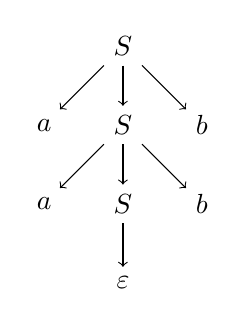
\begin{tikzpicture}
    \node (0){$S$};
    \node (2)[below of = 0]{$S$};
    \node (7)[below of = 2]{$S$};
    \node (5)[below of = 7]{$\varepsilon$};
    \node (1)[left of = 2]{$a$};
    \node (3)[right of = 2]{$b$};
    \node (4)[left of = 7]{$a$};
    \node (6)[right of = 7]{$b$};
    \draw[->] 
        (0) edge (1)
        (0) edge (2)
        (0) edge (3)
        (2) edge (4)
        (2) edge (6)
        (2) edge (7)
        (7) edge (5)
        ;
\end{tikzpicture}

\textbf{Определение.} КС-грамматика называется \textit{однозначной}, если для каждого слова $w$ существует ровно одно правостороннее дерево вывода для слова $w$.

\textbf{Определение.} Существенно неоднозначный КС-язык --- язык, для которого не существует однозначной КС-грамматики.

\textbf{Утверждение.} КС-языки замкнуты относительно:
\begin{itemize}
    \item Объединения: $S \to S_1$, $S \to S_2$.
    \item Конкатенации: $S \to S_1S_2$.
    \item Итерации Клини: $S \to S_1S$, $S \to \varepsilon$.
\end{itemize}
Про остальные операции позже.

\section{Нормальная форма Хомского}
\textbf{Определение.} КС-грамматика $G$ \textit{находится в нормальной форме Хомского}, если её правила имеют один из следующих видов:
\begin{itemize}
    \item $A \to a$, где $A \in N, a \in \Sigma$.
    \item $A \to BC$, где $A \in N$; $B, C \in N \setminus \{S\}$.
    \item $S \to \varepsilon$.
\end{itemize}

\textbf{Теорема.} Для любой КС-грамматики $G$ существует КС-грамматика $G_7$ в нормальной форме Хомского, такая что $L(G) = L(G_7)$.
Откуда 7? В алгоритме будет 7 шагов.

\subsection{Шаг 1: удаление непорождающих символов}
\textbf{Определение.} Символ $y \in N$ называется \textit{порождающим}, если существует слово $w \in \Sigma^*$, которое выводится из $y$.

Пусть $G_1$ --- грамматика $G$ без непорождающих символов.
Докажем, что $L(G) = L(G_1)$.
$L(G_1) \subset L(G)$ --- очевидно. В обратную сторону: пусть $w \in L(G) \setminus L(G_1)$.
Как это могло произойти? В случае, если $S \vdash \phi A \psi \vdash w$, где $A$ --- непорождающий.
Тогда $w = w_1 u w_2$, где $\phi \vdash w_1$, $\psi \vdash w_2$ и $A \vdash u$, то есть из $A$ всё-таки что-то вывели.
Можно сделать поиском в ширину по обратным рёбрам: запускаемся из всех терминалов и добавляем в очередь те нетерминалы, из которых можно вывести строку $\alpha \in (N \cup \Sigma)^*$, состоящую из терминалов и порождающих символов.

Время работы: $O(|P|)$.

\subsection{Шаг 2: удаление недостижимых символов}
\textbf{Определение.} Символ $D \in N$ называется \textit{достижимым}, если существует $\phi, \psi \in (N \cup \Sigma)^*$, такие что $S \vdash \phi D \psi$.

Удаляем недостижимые символы, получаем грамматику $G_2$.
Нужно доказать две вещи: грамматики совпадают и не появились непорождающие символы.

Первое. $L(G_2) \subset L(G_1)$ очевидно. Обратно, пусть $w \in L(G_1) \setminus L(G_2)$.
Тогда существует недостижимый $B$, такой что $S \vdash \phi B \psi \vdash w$, то есть $B$ достижим.

Второе. Пусть $B$ стал непорождающим, но он достижим.
Тогда существует недостижимый $C$, такой что $B \vdash \phi C \psi \vdash w$, то есть $C$ достижим.

Тоже делается поиском в ширину за $O(|P|)$.

\subsection{Шаг 3: удаление смешанных правил}
\textbf{Определение.} Правило \textit{смешанное}, если в правой части есть и терминал, и нетерминал.

Будем для каждого смешанного правила $A \to BcDe$ ставить правила $A \to BCDE$, $C \to c$ и $E \to e$.
Доказательство корректности --- в качестве упражнения.

Время работы --- $O(|P|)$.

\subsection{Шаг 4: длинные правила}
Вместо правила $A \to A_1A_2A_3A_4$ сделаем правила $A \to A_1C_1$, $C_1 \to A_2C_2$, $C_2 \to A_3C_3$, $C_3 \to A_3A_4$.
Корректность очевидна.

Время работы --- $O(|P|)$.

\subsection{Шаг 5: удаление $\varepsilon$-порождающих}
\textbf{Определение.} $A \in N$ называется $\varepsilon$-\textit{порождающим}, если $A \vdash \varepsilon$.
Их можно найти аналогично порождающим символам.

\textbf{Алгоритм.} Если $(A \to BC) \in P$ и $C \vdash \varepsilon$, то добавим правило $A \to  B$. Аналогично добавим $A \to C$ при необходимости.
После этого удалим все правила вида $E \to \varepsilon$.
Полученную грамматику обзовём $G_5$.

\textbf{Утверждение.} $L(G_5) = L(G_4) \setminus \{\varepsilon\}$.

\textbf{Доказательство.} Будем доказывать вложение в обе стороны.

$(L(G_4) \setminus \{\varepsilon\}) \subset L(G_5)$: индукцией по длине вывода.
Пусть $A \vdash_{G_4} w \ne \varepsilon$.
База: если $w$ --- буква, то такие правила мы не трогали, так что $A \vdash_{G_5} w$.

Переход: пусть $A \vdash_{G_4, 1} BC \vdash_{G_4} w_1 w_2 = w$ (случай $A \vdash_{G_4, 1} B \vdash_{G_4} w$ аналогичен).
Рассмотрим случаи:
\begin{enumerate}
    \item $w_1 \ne \varepsilon$, $w_2 \ne \varepsilon$, тогда по предположению индукции $B \vdash_{G_5} w_1$ и $B \vdash_{G_5} w_2$, поэтому $A \vdash_{G_5} BC \vdash_{G_5} w_1w_2 = w$.
    \item $w_1 = \varepsilon$. Тогда $B$ --- $\varepsilon$-порождающий и $(A \to C) \in P(G_5)$ (правила $G_5$). 
        По предположению индукции имеем $C \vdash_{G_5} w_2$, поэтому $A \vdash_{G_5} C \vdash_{G_5} w_2 = w$.
    \item $w_2 = \varepsilon$ --- аналогично.
\end{enumerate}

$(L(G_4) \setminus \{\varepsilon\}) \supset L(G_5)$: вновь индукцией по длине вывода. Пусть $A \vdash_{G_5} w$.
База аналогична, переход:
\begin{enumerate}
    \item $A \vdash_{G_5, 1} BC \vdash_{G_5} w_1w_2 = w$, где $B \vdash_{G_5} w_1$ и $C \vdash_{G_5} w_2$.
        Тогда по предположению индукции $B \vdash_{G_4} w_1$ и $C \vdash_{G_4} w_2$ и $BC \vdash_{G_4} w$.
    \item $A \vdash_{G_5, 1} B \vdash_{G_5} w$. 
        По предположению индукции $B \vdash_{G_4} w$.
        Как могло появиться правило $(A \to B) \in P(G_5)$? 
        Либо оно было в $G_4$, либо $A \vdash_{G_4} BD$, где $D \vdash_{G_4} \varepsilon$, либо то же самое для $A \vdash_{G_4} DB$.
        В первом случае всё очевидно, второй: $A \vdash_{G_4} BD \vdash_{G_4} B \vdash_{G_4} w$.
\end{enumerate}

\QED

Время работы: $O(|P|)$.

\subsection{Шаг 6: добавление $S \to \varepsilon$}
Заводим новый нетерминал $S'$ и делаем его стартовым.
Добавляем правило $S' \to S$ и, если $S \vdash \varepsilon$, добавим $S' \to \varepsilon$.

\subsection{Шаг 7: удаление унарных правил}
\textbf{Определение.} Унарное правило --- правило вида $A \to B$.

Если у нас есть цепочка $A_1 \to A_2 \to \dots \to A_k$, то просто сожмём промежуточные состояния аналогично удалению $\varepsilon$-переходов в автомате.

Время работы: $O(|P| \cdot |N|)$.

\subsection{Применение}
\textbf{Замечание.} Первые два шага нужны были просто для того, чтобы ``убрать мусор``.

Важное практическое применение --- Алгоритм Кока-Янгера-Касами проверки принадлежности слова грамматике. 
Заведём динамику $dp[A][i][j]$ --- правда ли, что можно вывести подотрезок $[i, j]$ слова $w$ из символа $A$. 
Засчёт НФ Хомского нам достаточно пытаться разбить отрезок только на два подотрезка, так что получается обычная динамика по подотрезкам.
Это самый простой алгоритм, работающий за $O(|N|^3 |P|)$.

\textbf{Лемма.} (О разрастании) Пусть $L$ --- КС-язык. Тогда
\[
    \exists p: \forall w \in L: |w| \ge p~ \exists x, u, y, v, z \in \Sigma^*: w = xuyvz, |uv| > 0, |uyv| \le p,
\]
\[
    \forall k \in \mathbb N~xu^kyv^kz \in L.
\]

\textbf{Доказательство.} Пусть $G$ --- грамматика, задающая $L$, в нормальной форме Хомского, $p = 2^{|N|}$ (множество нетерминалов).
Положим $h(w)$ --- высота дерева вывода слова $w$.
Тогда если $|w| = 1$, то $h(w) = 1$, если $|w| = 2$, то $h(w) \ge 2$, и в общем случае $h(w) \ge \log_2(|w|) + 1$.
Возьмём слово $w$, такое что $|w| \ge p$.
Так как $|w| \ge 2^{|N|}$, $h(w) \ge |N| + 1$, то есть существует нетерминал $A$, который встречается дважды при выводе одного символа.
Возьмём самый глубокий такой нетерминал.
Пусть мы прошли по цепи $S \vdash xAz \vdash xuAvz \vdash xuyvz$, то есть $A \vdash uAv \vdash uyv$.
Так как этот нетерминал самый глубокий из повторяющихся, в выводе $A \vdash uyv$ все нетерминалы на каждом пути от $A$ до терминала различны, иначе мы бы нашли повторяющийся глубже $A$.
Следовательно, аналогично рассуждениям выше $|uyv| \le 2^{|N|} = p$.

\QED

\textbf{Пример.} $\{a^nb^nc^n: n \in \mathbb Z^+\}$ не является контекстно-свободным.
Возьмём $p$ из леммы и слово $w = a^pb^pc^p$, тогда $w = xuyvz$, и $|uyv| \le p$, поэтому в $uyv$ не могут быть три различные буквы.
Из этого тривиально строится противоречие.

\textbf{Следствие 1.} КС-языки не замкнуты относительно пересечения, так как $\{a^nb^nc^n\} = \{a^nb^nc^k\} \cap \{a^kb^nc^n\}$.

\textbf{Следствие 2.} КС-языки не замкнуты относительно дополнения. Пример: $\Sigma^* \setminus \{a^nb^nc^n\}$.

\section{Алгоритм Эрли}
Ещё один алгоритм проверки принадлежности слова КС-грамматике.

\textbf{Определение.} Ситуация --- $(A \to \alpha \cdot \beta, i, j)$, где $i, j \in [0, |w|]$, $i$ --- позиция родителя, $j$ --- текущая позиция в дереве обхода, $A \to \alpha \beta$ --- правило грамматики, $\cdot$ --- текущая позиция в разборе правила.

\textbf{Определение.} Ситуация $(A \to \alpha \cdot \beta, i, j)$ \textit{достижима}, если она выводится алгоритмом Эрли. $D_j$ --- множество всех достижимых ситуаций с фиксированным $j$.

Соответственно смысл алгоритма заключается в том, чтобы постепенно найти все достижимые ситуации. Для этого используются следующие операции:
\begin{itemize}
    \item Scan: мы находимся в ситуации $(A \to \alpha \cdot a \beta, i, j)$ и $w_j = a$.
        Тогда можно подвинуть текущую позицию и перейти в $(A \to \alpha a \cdot \beta, i, j + 1)$.
        Название следует из того, что мы считываем один символ.
    \item Predict: войти в поддерево. Пусть ситуация $(A \to \alpha \cdot B \beta, i, j)$ достижима. 
        Тогда для всех правил $B \to \gamma$ мы объявляем достижимыми ситуации $(B \to \cdot \gamma, j, j)$.
    \item Complete: выйти из поддерева. Если $(B \to \gamma \cdot, k, j) \in D_j$ и $(A \to \alpha \cdot B \beta, i, k) \in D_k$, то объявляем $(A \to \alpha B \cdot \beta, i, j) \in D_j$.
\end{itemize}

Как можно заметить из переходов, чтобы найти все достижимые ситуации, достаточно перебирать все $D_j$ в порядке возрастания $j$: если мы найдём новую достижимую ситуацию, то она точно не будет в предыдущих множествах.
Соответственно так и будем перебирать все множества $D_j$, а в них --- ситуации, пытаясь из каждой сделать Scan, Predict и Complete.
(Изначально достижима ровно одна ситуация --- $(S' \to \cdot S, 0, 0)$)

\subsection{Корректность}
Пока что непонятно, какую связь ситуации имеют с выводимостью слова в грамматике. Её устанавливает следующая

\textbf{Лемма.} Cитуация $(A \to \alpha \cdot \beta, i, j)$ достижима тогда и только тогда, когда $\exists \psi \in (N \cup \Sigma)^*, \alpha \vdash w[i,j)$, такие что $S' \vdash w[0,i) A \psi \vdash_1 w[0,i) \alpha \beta \psi$.
Иными словами, существует вывод, при котором мы выводим $w[0,i)A$, как подстроку, и после можем раскрыть до $w[0,i) \alpha \beta \vdash w[0,j) \beta$.

Мотивация леммы --- достижимость ситуации $(S' \to S \cdot, 0, |w|)$ (подробнее после доказательства).

\textbf{Доказательство.} $\Rightarrow$. Индукцией по количеству шагов в алгоритме. База: $(S' \to \cdot S, 0, 0)$ --- стартовая ситуация.
Тогда, подставляя $i = 0$, $\alpha = \psi = \varepsilon$, получаем $S' \vdash w[0,0) S' \varepsilon \vdash_1 \cdot S$.
Переходы.
\begin{itemize}
    \item Scan. После него будет $(A \to \alpha \cdot \beta, i, j + 1)$.
        Тогда была ситуация $(A \to \alpha \cdot a\beta, i, j)$ и $w_j = a$.
        По предположению индукции $S' \vdash w[0,i) A \psi \vdash_1 w[0,i) \alpha \beta \psi$, так что $\alpha \vdash[i,j)$.
        Тогда $\alpha a \vdash w[i,j + 1)$ --- берём в качестве нового $\alpha$.
    \item Predict: пусть мы перешли из $(A \to \alpha \cdot B \gamma, i, j)$ с правилом $B \to \beta$ в ситуацию $(B \to \cdot \beta, j, j)$.
        По предположению индукции $\exists \psi: \alpha \vdash w[i, j)$, такое что $S' \vdash w[0, i) A \psi \vdash_1 w[0, i) \alpha B \gamma \psi$.
        Так как $\alpha \vdash w[i, j)$, $S' \vdash w[0, j) B \gamma \psi \vdash_1 w[0, j) \beta \gamma \psi$.
        Теперь берём в утверждении $\alpha = \varepsilon$, $\beta = \beta$, $\psi = \gamma \psi$ и получаем искомое.
    \item Scan: пусть у нас есть ситуации $(B \to \gamma \cdot, k, j)$ и $(A \to \alpha \cdot B \beta, i, k)$.
        Из предположения индукции $\gamma \vdash w[k, j)$, $\alpha \vdash w[i, k)$, $\exists \psi_1, \psi_2: S' \vdash w[0, k) B \psi_1 \vdash_1 w[0, k) \gamma \psi_1$ и $S' \vdash w[0, i) A \psi_2 \vdash_1 w[0, i) \alpha B \beta \psi_2$.

        Хотим для ситуации $(A \to \alpha B \cdot \beta, i, j)$ найти $\psi_3$ и доказать $\alpha B \vdash w[i, j)$.
        Первое очевидно: $\psi_3 = \psi_2$.
        Второе тривиально: $\alpha B \vdash \alpha \gamma \vdash w[i, j)$.
        
\end{itemize}

$\Leftarrow$. Будем делать индукцию по тройке $(j, k + e, e)$ в лексикографическом порядке, где $j$ --- позиция, $k + e$ --- длина полного вывода до $j$, $e$ --- длина вывода от $i$ до $j$.
База: $S' \vdash_0 w[0,i) A \psi$, тогда $i = 0$, $A = S'$ и $\psi = \varepsilon$.
Дальше: $w[0,i) A \psi \vdash_1 w[0,i) \alpha \beta \psi \vdash_0 w[0,i) w[i,0) \beta \psi$.
То есть $\alpha \vdash_0 w[i,0)$, поэтому $\alpha = \varepsilon$ и $\beta = S$.
Берём ситуацию $(S' \to \alpha \cdot \beta, 0, 0) = (S' \to \cdot S, 0, 0)$, которая у нас уже есть.

Переход. Пусть $S' \vdash w[0,i) A \psi \vdash_1 w[0,i) \alpha \beta \psi$ и $\alpha \vdash_l w[i,j)$.
Рассмотрим последний символ $\alpha$. Возможны три случая:
\begin{itemize}
    \item $\alpha = \alpha' b$. Тогда $\alpha' \vdash w[i,j-1)$ и $w_{j-1} = b$.
        Применим предположение индукции к переходу $A \to \alpha' (b\beta)$ с тройкой $(j - 1, k + l, l)$, получаем ситуацию $(A \to \alpha' \cdot b \beta, i, j - 1)$.
        Тогда ситуацию $(A \to \alpha' b \cdot \beta, i, j)$ можно получить через Scan.
    \item $\alpha = \alpha' B$. Рассмотрим дерево разбора: можно увидеть, что $\alpha' \vdash_t w[i,p)$, и, так как $w[i,j)$ выводится на $l$ шагов, $B \vdash_1 \gamma \vdash_{l-t-1} w[p,j)$.
        Тогда, применяя предположение индукции для перехода $B \to \gamma \varepsilon$ и тройки $(j, k + l, l - t - 1)$, получаем ситуацию $(B \to \gamma \cdot, p, j)$.
        Применяя предположение к правилу $A \to \alpha' (B \beta)$ с тройкой $(p, k + t, t)$, получаем ситуацию $(A \to \alpha' \cdot B \beta, i, p)$, поэтому по операции Complete получаем ситуацию $(A \to \alpha'B \cdot \beta, i, j)$.
    \item $\alpha = \varepsilon$. Имеем $S' \vdash w[0, i)A \psi$. Посмотрим на нетерминал, который вывел $A$: $S' \vdash w[0, p) B \psi'$ и существует правило $B \to \gamma A \phi$.
        Тогда $\gamma \vdash_t w[p, i)$.
        Применяем предположение индукции к $B \to \gamma (A\phi)$ с тройкой $(i, k - 1, t)$ (второй элемент --- $k - 1$, так как это момент до раскрытия $A$).
        Получаем ситуацию $(B \to \gamma \cdot A \phi, p, i)$ и, делая Predict с переходом $A \to \varepsilon \beta$, приходим в $(A \to \cdot \beta, i, i)$.
\end{itemize}

\QED

\textbf{Корректность алгоритма.} $w \in L(G) \iff S' \vdash_1 S \vdash w[0,0)S \vdash w[0,|w|)$.
Применяя лемму, получаем, что это происходит тогда и только тогда, когда ситуация $(S' \to S, 0, |w|)$ достижима, то есть когда алгоритм возвращает \verb+true+.

\subsection{Асимптотика в общем случае}
Рассмотрим количество ситуаций для конкретного $j$.
Количество правил --- $O(|G|)$, кандидатов в $i$ --- $O(|w|)$, поэтому $|D_j| = O(|w| \cdot |G|)$, где $|G|$ --- суммарное число символов во всех левых частях правил.

\textbf{Определение.} $D_j[\gamma]$ --- правила вида $(A \to \alpha \cdot \gamma, i, j)$.

Асимптотика Scan-а: просто перебираем все $D_j[\gamma]$ для фиксированного $j$, получается $O(|w| \cdot |G|)$.

Predict-а: перебираем все правила $B \to \gamma$ и для каждого рассмотрим $D_j[B]$. Получается суммарно $O(|w| \cdot |G|^2)$.

Complete-а: перебираем все ситуации с фиксированной позицией $i$, то есть $O(|w|^2 \cdot |G|^2)$.

Следовательно, суммарно по всем позициям получается $O(|w|^3 \cdot |G|^2)$.

\subsection{Асимптотика для однозначных грамматик}
Утверждается, что если грамматика однозначна, то алгоритм Эрли работает за $O(|w|^2 \cdot |G|^2)$. Понятно, что достаточно улучшить оценку для Complete-ов, чем мы сейчас и займёмся.
Дополнительно удалим непорождающие нетерминалы, всё равно это предподсчёт.

\textbf{Лемма.} Пусть $\alpha \ne \varepsilon$. Тогда алгоритм Эрли будет пытаться добавить ситуацию $(A \to \alpha \cdot \beta, i, j)$ в $D_j$ не более одного раза.

\textbf{Доказательство.} Рассмотрим все моменты времени, когда была попытка добавить эту ситуацию.
Если $\alpha = \alpha' a$, то она могла быть добавлена только Scan-ом, причём только из ситуации $(A \to \alpha' \cdot a \beta, i, j - 1)$.

Теперь пусть $\alpha = \alpha' B$, ситуация могла быть добавлена только Complete-ом. 
Допустим, что было хотя бы две попытки из различных пар ситуаций:
\[
    \begin{cases}
        (A \to \alpha' \cdot B \beta, i, k_1) \in D_{k_1} \\
        (B \to \gamma_1 \cdot, k_1, j) \in D_j
    \end{cases}
    \begin{cases}
        (A \to \alpha' \cdot B \beta, i, k_2) \in D_{k_2} \\
        (B \to \gamma_2 \cdot, k_2, j) \in D_j
    \end{cases}
\]
Заметим, что $\alpha' \gamma_1 \vdash w[i, j)$ и $\alpha' \gamma_2 \vdash w[i, j)$.
Так как мы удалили непорождающие символы, существуют $\psi$ и $\phi$, такие что $S' \vdash \phi \alpha' \gamma_1 \psi \vdash w[0, j) \psi \vdash w[0, j')$ и $S' \vdash \phi \alpha' \gamma_2 \psi \vdash w[0, j) \psi \vdash w[0, j')$.
Получаем, что если $k_1 \ne k_2$ или $\gamma_1 \ne \gamma_2$, то у строки $w[0, j')$ будет два различных дерева вывода --- противоречие с однозначностью.

\QED

Ещё раз вспомним, как мы оценивали Complete.
Мы перебираем все ситуации $(A \to \alpha \cdot \beta, i, j)$ в $D_j$ и для каждой из них перебираем все ситуации $(B \to \gamma \cdot, j, k)$, где $\beta = B \beta'$ (список таких ситуаций можно поддерживать, чтобы не тратить время на поиск).
Каждая пара ситуаций будет инициировать попытку добавления ситуации в $D_k$, поэтому по лемме мы суммарно переберём не более $\sum_{k=1}^{|w|} D_k$ пар, что является $O(|w|^2 |G|)$.

\section{МП-автоматы}
\textbf{Определение.} Автомат с магазинной памятью (МП-автомат) --- это $M = \left< Q, \Sigma, \Gamma, \Delta, q_0, F \right>$, где:
\begin{itemize}
    \item $Q$ --- конечное множество состояний.
    \item $\Sigma$ --- конечный алфавит.
    \item $\Gamma$ --- стековый (внутренний) алфавит, тоже конечен и не пересекается с $\Sigma$.
    \item $\Delta \subset (Q, \Sigma^*, \Gamma^*) \times (Q, \Gamma^*)$ --- конечное множество переходов (пишем строку из $\Sigma$, снимаем со стека строку из $\Gamma$, кладём на стек строку из $\Gamma$).
    \item $q_0 \in Q$ --- стартовое состояние.
    \item $F \subset Q$ --- завершающие состояния.
\end{itemize}
Изначально стек пустой, для завершения чтения слова он тоже должен быть пуст.

\textbf{Определение.} Конфигурция МП-автомата --- тройка $\left<q, u, \gamma \right>$: находимся в состоянии $q$, осталось прочитать слово $u$, на стеке лежит $\gamma$.

\textbf{Определение.} Выводимость --- наименьшее рефлексивное транзитивное отношение, такое что для любого перехода $\left<q, u, \alpha \right> \to \left<q_2, \beta \right>$ и для любых $v \in \Sigma^*, \eta \in \Gamma^*$ выполнено $\left< q_1, uv, \eta \alpha \right> \vdash \left< q_2, v, \eta \beta \right>$ (то есть читаем префикс слова и меняем суффикс стека).

\textbf{Определение.} Язык, распознаваемый МП-автоматом --- это $L(M) = \{v~|~ \exists q \in F: \left< q_0, v, \varepsilon \right> \vdash \left< q, \varepsilon, \varepsilon \right>\}$.

\textbf{Пример.} Следующие языки можно задать МП-автоматами:
\begin{itemize}
    \item $\{a^n b^n~|~n \in \mathbb N\}$.
    \item $\{w~|~|w|_a = |w|_b\}$ --- здесь нужно поддерживать баланс, его можно эмулировать стеком: если на стеке $n$ букв $A$, то баланс --- $+n$, если $n$ букв $B$, то --- $-n$.
\end{itemize}

\textbf{Теорема.} Для любого МП-автомата $M$ существует эквивалентный автомат $M'$, такой что для любого перехода $\left<q_1, u, \alpha \right> \to \left< q_2, \beta \right>$ верно $|u| \le 1$ и $|\alpha| + |\beta| \le 1$ --- не более, чем однобуквенные переходы.

\textbf{Доказательство.} Возьмём такой переход и надобавляем промежуточных вершин так, чтобы сначала считать слово по одному символу, потом по одной снять буквы со стека и, наконец, по одной положить буквы на стек.

\QED

Как может показаться из примеров, МП-автоматы могут быть эквивалентны КС грамматикам. 
И это правда, дальше будем это доказывать.
\subsection{Автомат ``перенос-свёртка``}
Возьмём КС грамматику $G = \left<N, \Sigma, P, S\right>$ и построим МП-автомат по следующему принципу (неформально): внутренний алфавит --- $N \cup \Sigma$, внешний --- $\Sigma$.
На стеке у него будут лежать правые части правил, и при переходах они будут заменяться на соответствующие левые части.
Также добавим переход считывания символа, не трогая стек.
Соответственно, если на стеке остался только $S$, то мы успешно прочитали слово.

Теперь формально: построим автомат $M = \{\{q_0, q_1\}, \Sigma, N \cup \Sigma, \Delta, q_0, \{q_1\}\}$, где $\Delta$ состоит из правил вида:
\begin{itemize}
    \item $\left<q_0, \varepsilon, S \right> \to \left< q_1, \varepsilon \right>$ --- завершающее условие, когда всё считали.
    \item $\left<q_0, \varepsilon, \alpha \right> \to \left< q_0, A \right>$ для всех правил $(A \to \alpha) \in P$ --- сворачивание правила, Reduce.
    \item $\left<q_0, a, \varepsilon \right> \to \left<q_0, a \right>$ для всех $a \in \Sigma$ --- считывание символа, Shift.
\end{itemize}

Остаётся доказать, что такой автомат эквивалентен грамматике $G$. А именно, необходимо доказать следующие два факта:

\textbf{Теорема.}
\begin{itemize}
    \item $A \vdash_G w \iff \left<q_0, w, \varepsilon \right> \vdash_M \left< q_0, \varepsilon, A \right>$ --- из нетерминала выводимость эквивалентна.
    \item $a \vdash_G w \iff \left<q_0, w, \varepsilon \right> \vdash_M \left< q_0, \varepsilon, a \right>$ --- из терминала выводимость эквивалентна.
\end{itemize}

\textbf{Доказательство.}
$\Rightarrow$. Пусть $\alpha$ --- однобуквенный терминал/нетерминал. Докажем индукцией по длине вывода.
База: $\alpha \vdash_0 w$ --- верно только при $\alpha = w \in \Sigma$, переход $\left<q_0, a, \varepsilon \right> \to \left<q, \varepsilon \right>$ мы добавляли.

Переход: теперь уже $\alpha = A$ --- нетерминал. Пусть $A \vdash_1 \alpha_1 \dots \alpha_k \vdash w_1 \dots w_k = w$.
Применяя предположение индукции ко всем $\alpha_i$, получаем $\left<q_0, w_i, \varepsilon \right> \vdash \left<q_0, \alpha_i \right>$.
Теперь у нас есть переход для правила $A \to \alpha_1 \dots \alpha_k$, поэтому $\left<q_0, \varepsilon, \alpha_1 \dots \alpha_k \right> \vdash \left<q_0, \varepsilon, A \right>$.
Собирая вместе, получаем $\left< q_0, w, \varepsilon \right> \vdash \left<q_0, \varepsilon, \alpha_1 \dots \alpha_k \right> \vdash \left<q_0, \varepsilon, A \right>$.

$\Leftarrow$. Опять же индукцией по длине вывода. 
База. Ноль шагов быть не может, поэтому начинаем с одного шага:
$\left<q_0, w, \varepsilon \right> \vdash_1 \left<q_0, \varepsilon, \alpha \right>$.
Если $\alpha = a$, то по рефлексивности верно. Иначе $\alpha = A$, тогда $w = \varepsilon$ (в противном случае такого перехода нет) и этот переход соответствует правилу $A \to \varepsilon$.

Переход: $\left<q_0, w, \varepsilon \right> \vdash \left<q_0, \varepsilon, \alpha_1 \dots \alpha_k \right> \vdash_1 \left<q_0, \varepsilon, A \right>$ --- вновь должен быть нетерминал $\alpha = A$.
Последний переход есть в грамматике по построению, а всё остальное выводится по предположению индукции (только нужно аккуратно выделить моменты времени, когда символы $\alpha_i$ появляются на стеке).

\QED

Теперь остаётся доказать эквивалентность построенного автомата и грамматики. Рассмотрим слово $w$, тогда имеет место следующая цепочка эквивалентных утверждений:
\begin{itemize}
    \item $w \in L(M)$.
    \item $\left<q_0, w, \varepsilon \right> \vdash \left<q_0, \varepsilon, \varepsilon \right>$ (определение штопора).
    \item $\left<q_0, w, \varepsilon \right> \vdash \left<q_0, \varepsilon, S \right>$ (так как есть соответствующий переход из $\left<q_0, \varepsilon, S \right>$.
    \item $S \vdash w$ (по теореме).
    \item $w \in L(G)$ (по определению штопора у грамматик).
\end{itemize}

\subsection{Грамматика по автомату}
Рассмотрим МП-автомат, у которого при каждом переходе либо добавляется на стек, либо снимается со стека \textbf{ровно} один символ.
У него есть переходы двух типов:
\begin{enumerate}
    \item $\left<q_i, u, \varepsilon \right> \to \left<q_j, A\right>$ для, возможно, пустого слова $u$ и $A \in \Gamma$.
    \item $\left<q_i, u, A \right> \to \left<q_j, \varepsilon \right>$ аналогично.
\end{enumerate}
Заметим, что при выводе слова мы всегда можем взаимно однозначно каждому переходу первого типа сопоставить переход второго типа.
Из этих соображений построим КС грамматику на множестве пар состояний автомата: $N = \{A_{i,j}~|~q_i,q_j \in Q\} \cup \{S\}$
Теперь добавим правила вывода на основе выделения пары переходов, которые добавляют и снимают один и тот же символ.
А именно, если в автомате есть переходы $\left<q_i, u, \varepsilon \right> \to \left<q_s, A \right>$ и $\left<q_t, v, A \right> \to \left<q_r, \varepsilon \right>$, то для всех $j$ мы можем попробовать прийти из $i$ в $j$, используя два перехода выше.
Иными словами, добавляем правило $A_{i,j} \to u A_{s,t} v A_{r,j}$.
Таким образом, мы считали $u$, добавив $A$ на стек, прошли из $s$ в $t$ так, чтобы по итогу стек не изменился, сняли $A$, считав $v$, и дошли до $j$.
Остаётся добавить правила $A_{i,i} \to \varepsilon$, чтобы символы что-нибудь порождали, и $S \to A_{0,j}$ для всех завершающих $q_j$.

По итогу вывод слова в этой грамматике выглядит примерно так: фиксируем конечное состояние $q_j$, переходим в $A_{0,j}$, выбираем путь из $q_0$ в $q_j$, разбиваем его на отрезки, не изменяющие стек, и соответствующими правилами вывода получаем этот путь.
Остаётся всего лишь показать эквивалентность этой грамматики автомату.

\textbf{Теорема.} $A_{i,j} \vdash w \iff \left<q_i, w, \varepsilon \right> \vdash \left<q_j, \varepsilon, \varepsilon \right>$.

\textbf{Доказательство.} Индукцией по длине вывода. 

$\Rightarrow$. База: 1 шаг, то есть $A_{i,j} \vdash_1 w$.
Тогда $w = \varepsilon$, такое может быть только при $i = j$, очевидно.

Переход: $A_{i,j} \vdash_1 uA_{s,t} v A_{r,j} \vdash u w_1 v w_2$.
По предположению $\left<q_s, w_1, \varepsilon \right> \vdash \left<q_t, \varepsilon, \varepsilon \right>$ и $\left<q_r, w_2, \varepsilon \right> \vdash \left<q_j, \varepsilon, \varepsilon \right>$.
Так как первый переход существует, $\left<q_i, u, \varepsilon \right> \vdash \left<q_s, \varepsilon, \varepsilon \right>$ и $\left<q_t, v, \varepsilon \right> \vdash \left<q_r, \varepsilon, \varepsilon \right>$.
Остаётся собрать всё в один переход.

$\Leftarrow$. База: 0 шагов, $\left<q_i, w, \varepsilon \right> \vdash_0 \left<q_j, \varepsilon, \varepsilon \right>$ --- верно только при $i = j$ и $w = \varepsilon$, такой переход имеется.

Переход: $\left<q_i, w_1 w_2 w_3 w_4, \varepsilon \right> \vdash_1 \left<q_s, w_2 w_3 w_4, A \right> \vdash \left<q_t, w_3 w_4, A \right> \vdash_1 \left<q_r, w_4, \varepsilon \right> \vdash \left<q_j, \varepsilon, \varepsilon \right>$ --- после первого перехода $q_i \to q_s$ должно было что-то появиться на стеке, потом это что-то должно было сняться в каком-то переходе $q_t \to q_r$, после чего можно смело идти до конца.
Остаётся применить предположение индукции: $A_{s,t} \vdash w_2$, $A_{r, j} \vdash w_4$, а для оставшихся переходов мы специально строили правило: $A_{i,j} \vdash w_1 A_{s,t} w_3 A_{r,j} \vdash w_1 w_2 w_3 w_4 = w$.

\QED

Для доказательства эквивалентности остаётся написать цепочку равносильных утверждений:
\begin{itemize}
    \item $w \in L(M)$.
    \item $\exists q_f \in F: \left<q_0, w, \varepsilon \right> \vdash \left<q_f, \varepsilon, \varepsilon \right>$.
    \item $\exists q_f \in F: A_{0,f} \vdash w$.
    \item $S \vdash w$.
    \item $w \in L(G)$.
\end{itemize}

\section{Нормальная форма Грейбах}
\textbf{Мотивация.} КС грамматики прекрасны, но есть одна проблема: выводить слова довольно тяжело из-за того, что мы не можем знать наверняка, какой первый символ может получиться из данного нетерминала, и для вывода первого символа приходится раскрывать первые нетерминалы.
Нормальная форма Грейбах решает эту проблему: при раскрытии любого нетерминала мы точно знаем первый символ.
В частности, с помощью такой грамматики можно будет построить МП-автомат без $\varepsilon$-переходов.

\textbf{Определение.} КС грамматика находится в \textit{нормальной форме Грейбах}, если все её правила имеют один из следующих видов ($a \in \Sigma$, $A \in N$ и $B, C \in N \setminus \{S'\}$).
\begin{itemize}
    \item $A \to a$.
    \item $A \to aB$.
    \item $A \to aBC$.
    \item $S' \to \varepsilon$.
\end{itemize}

\subsection{Построение}
Будем переводить грамматику из НФ Хомского в НФ Грейбах.
Для этого мы будем строить новую грамматику на нетерминалах вида $B \setminus A$ --- аналог левого деления. 
Хочется сделать так, чтобы $B \setminus A \vdash w \iff A \vdash Bw$.
То есть из $B \setminus A$ выводятся слова из $A$ с отрезанным префиксом из $B$.
Теперь к построению самих переходов.
Пусть $A \vdash C\alpha \vdash_1 BD\alpha$, то есть $C$ --- нетерминал, из которого выводится $B$.
Теперь найдём первую букву, которая выводится из $D$: пусть $D \vdash E\beta \vdash_1 e\beta$.
Так, мы хотим, чтобы $B \setminus A \vdash e \beta \alpha$.
Тогда и добавим правило $B \setminus A \to e(E \setminus D)(C \setminus A)$ --- если у нетерминалов в правой части переходы корректны, то $E \setminus D \vdash \beta$ и $C \setminus A \vdash \alpha$, как и хотелось.
Теперь ещё для красоты добавим $A \setminus A \to \varepsilon$.

Однако у нас всё ещё нет правил раскрытия $S'$.
Добавим, при необходимости, правило $S' \to \varepsilon$, теперь научимся выводить непустое слово $w = aw'$, где $a \in \Sigma$, такое что $S \vdash w$.
Так как исходная грамматика была в НФ Хомского, существует нетерминал $A$, такой что $S \vdash Aw' \vdash_1 aw'$.
Соответственно остаётся добавить переход $S \to a(A \setminus S)$, и оно теперь тоже выводится.

Казалось бы, всё, но у нас же есть запрещённый переход $A \setminus A \to \varepsilon$, да и ещё нигде не используется переход $A \to aB$ (кроме случая $A = S$)...
Обе проблемы решаются удалением $\varepsilon$-порождающих нетерминалов.

Теперь ещё раз выпишем все построенные переходы и докажем, что мы построили то, что хотели:
\begin{itemize}
    \item $S' \to a(A \setminus S')$, если $(A \to a) \in P$.
    \item $A \setminus A \to \varepsilon$ для всех $A \in N$.
    \item $B \setminus A \to e(E \setminus D)(C \setminus A)$, если $(E \to e), (C \to BD) \in P$.
\end{itemize}

\textbf{Утверждение.} $B \setminus A \vdash w \iff A \vdash Bw$.

\textbf{Доказательство.} $\Leftarrow$: индукция по длине вывода + по построению.

$\Rightarrow$: снова индукция по длине вывода. База: $B \setminus A \vdash_1 w$, тогда $w = \varepsilon$ и $B = A$ --- верно.

Переход: $B \setminus A \vdash_1 e(E \setminus D)(C \setminus A) \vdash euv$, то есть $w = euv$.
По предположению индукции $D \vdash Eu$ и $A \vdash Cv$.
Так как переход из $B \setminus A$ существует, существуют и переходы $E \to e$ с $C \to BD$.
Получаем $D \vdash eu$ и $A \vdash BDv \vdash Beuv = Bw$.

\QED

\textbf{Теорема.} Полученная грамматика эквивалентна исходной.

\textbf{Доказательство.} Принадлежность $\varepsilon$ эквивалентна по построению. Теперь рассмотрим $w = au$, $a \in \Sigma$.
Цепочка эквивалентных утверждений:
\begin{itemize}
    \item $au \in L(G)$.
    \item $S \vdash au$.
    \item $\exists A \in N: S \vdash Au \vdash_1 au$.
    \item $\exists A \in N: S' \vdash a(A \setminus S)$, причём $S \vdash Au$ и $A \vdash a$.
    \item $S' \vdash au$ (так как $S \vdash Au \iff A \setminus S \vdash u$).
    \item $au \in L(G')$.
\end{itemize}

\QED

Остаётся убрать $\varepsilon$-переходы и получится грамматика в исходной форме.

\textbf{Замечание.} Грамматику можно аналогичным образом привести к \textit{обратной нормальной форме Грейбах}: в ней в правых частях правил терминальный символ стоит не первым, а последним.

\subsection{Применение}
При помощи НФ формы Грейбах можно по произвольному МП-автомату построить эквивалентный, у которого все переходы однобуквенные.
Для этого построим по нему КС грамматику, приведём её к \textbf{обратной} НФ Грейбах и по ней построим МП-автомат через перенос-свёртку.
Однако у построенного автомата всё ещё будут $\varepsilon$-переходы, ведь все сворачивания правил являются таковыми.
Но теперь вспоминаем, что у всех сворачиваний правил на конце есть терминал, и мы этот терминал должны были когда-то считать, чтобы сейчас снять его со стека.
Поэтому аналогично построению КС грамматики по МП-автомату мы можем выделить пары переходов, которые работают с одним терминалом, и свернуть их в один однобуквенный переход.
Доказательство, как и идея, аналогично.

Эта конструкция позволяет нам построить пересечение КС языка с автоматным.
Действительно, построим МП-автомат $M$ с однобуквенными переходами, НКА с однобуквенными переходами $P$ и рассмотрим их декартого произведение.
А именно, автомат $T = \left<Q_M \times Q_P, \Sigma, \Gamma, \Delta, (q_0^M, q_0^P), F_M \times F_P \right>$ с переходами $\left<(q_1, p_1), a, \alpha \right> \to \left<(q_2, p_2), \beta \right>$ для переходов в исходных автоматах $(\left<q_1, a \right> \to q_2) \in \Delta_M$ и $(\left<p_1, a, \alpha \right> \to \left<p_2, \beta \right>) \in \Delta_P$.
Иными словами, пересекаем автоматы и добавляем к ним стек.

Таким образом, мы ``доказали``, что пересечение КС языка и автоматного языка --- КС язык.

\section{LR алгоритм}
Алгоритм переноса-свёртки имеет недостаток того, что действия неоднозначны и тяжело понимать, что на стеке лежит правая часть правила.
Для этого введём ситуации из алгоритма Эрли. Главная идея алгоритма --- построить ДКА над множеством ситуаций, где переход по символу --- сдвиг точки, а по $\varepsilon$ --- раскрытие нетерминала.
Тогда мы будем пытаться считывать слово, пока есть соответствующие переходы в автомате, а если нет, то будем делать Reduce --- переход по $\varepsilon$ со сворачиванием нетерминала.

Неформально, $LR(k)$ --- это алгоритм перенос-свёртка, в котором для улучшения асимптотики мы дополнительно смотрим на $k$ букв вперёд.
В частности, $LR(0)$ --- это и есть почти алгоритм переноса-свёртки.

\textbf{Определение.} Символ конца слова --- \$.

\textbf{Определение.} 
\[
    \First(\alpha) = \{a~|~\alpha \vdash au, u \in \Sigma^*\} \cup \{\text{\$, если $\alpha \vdash \varepsilon$}\}.
\]
Иными словами, множество первых символов, выводимых из $\alpha$.

\textbf{Определение.} $LR(1)$ ситуация --- ситуация вида $(A \to \alpha \cdot \beta, a)$, где $a \in \Sigma \cup \{\$\}$, остальное, как в ситуациях Эрли.

\textbf{Соглашение.} До конца этого параграфа $\vdash_r~=~\vdash$ --- правосторонний вывод.

\textbf{Определение.} $\alpha$ --- активный префикс, если
\[
    \exists \alpha_1\beta_1 = \alpha: S' \vdash_r \alpha_1 Au \vdash_{r,1} \alpha_1 \beta_1 \beta_2 u.
\]
Как понять это определение: здесь именно принципиально, что вывод правосторонний, то есть после того, как строка $\alpha_1 \beta_1 \beta_2$ была получена из нетерминалов, в ней нетерминалы больше не раскрывались.
На самом деле, это в точности те слова, которые могут быть на стеке во время алгоритма переноса-свёртки.
В частности, префикс активного префикс сам является активным префиксом.

\textbf{Определение.} Ситуация $(A \to \beta_1 \cdot \beta_2, a)$ допустима для активного префикса $\alpha \beta_1$, если
\[
    S' \vdash \alpha Au \vdash_1 \alpha \beta_1 \beta_2 u, a \in \First(u).
\]
То есть это ситуации, которые \textit{допускают} появление данного активного префикса.

\textbf{Определение.} $\Adm(\alpha)$ --- множество всех допустимых ситуаций для активного префикса $\lambda$.

\textbf{Определение.} Замыкание множества ситуаций $I$ --- наименьшее множество $J \supset I$, такое что
\[
    \begin{cases}
        (B \to \gamma) \in P \\
        (A \to \alpha \cdot B \beta, a) \in J
    \end{cases}
    \Rightarrow (B \to \cdot \gamma, c) \in J~\forall c \in \First(\beta a).
\]
То есть наименьшее множество, которое замкнуто относительно операции Predict. Обозначение: $J = \CLOSURE(I)$.

\textbf{Определение.} Для $\lambda \in N \cup \Sigma$
\[
    \GOTO(I,\lambda) = \CLOSURE(A \to \alpha \lambda \cdot \beta, a~|~(A \to \alpha \cdot \lambda \beta, a) \in I).
\]
То есть ситуации из $I$ после считывания символа $\lambda$.


\textbf{Лемма 0.1.} Если $\alpha \vdash \beta$, то $\First(\beta) \vdash \First(\alpha)$.

\textbf{Лемма 0.2.} Пусть $\alpha \vdash u$. Тогда для любого $a \in \First(u \gamma)$ существует $b \in \First(\gamma)$, такой что $a \in \First(\alpha b)$.

\textbf{Доказательство.} Пусть $a \in \First(u \gamma)$.
Если $u = ax$, то $\alpha b \vdash ub \vdash axb$.
Иначе $u = \varepsilon$, тогда $a \in \First(\gamma)$.
В обоих случаях можно взять $b = a$.

\textbf{Лемма 1.} Если $I \subset \Adm(\alpha)$, то $\CLOSURE(I) \subset \Adm(\alpha)$.

\textbf{Доказательство.} Пусть $(A \to \beta_1 \cdot B \beta_2, a) \in I$ и $(B \to \gamma) \in P$.
Зафиксируем $c \in \First(\beta_2 a)$ и докажем, что ситуация $(B \to \cdot \gamma, c)$ лежит в $\Adm(\alpha)$.
По определению активного префикса
\[
    S' \vdash \alpha' Au \vdash_1 \alpha' \beta_1 B \beta_2 u,
\]
где $\alpha' \beta_1 = \alpha$ и $a \in \First(u)$.
Теперь раскроем $\beta_2$ и после этого $B$ (в таком порядке, ибо вывод правосторонний):
\[
    \alpha B \beta_2 u \vdash \alpha B vu \vdash_1 \alpha \gamma vu.
\]
Итак, мы получили, что
\[
    S' \vdash \alpha~B~vu \vdash_1 \alpha \varepsilon~\gamma~vu,
\]
то есть для доказательства допустимости $(B \to \cdot \gamma, c)$ осталось показать, что $c \in \First(vu)$.
Всё, что мы знаем про $c$, --- это $c \in \First(\beta_2 a)$, где $\beta_2 \vdash v$ и $a \in \First(u)$.
Здесь помогает факт, что $v$ мы выбираем сами.
Если существует $v = cx$, такое что $\beta_2 \vdash v$, то берём его, и тогда $c \in \First(v) = \First(vu)$.
В противном случае $\beta_2 \vdash \varepsilon$, тогда берём $v = \varepsilon$, и в этом случае $c = a \in \First(u) = \First(vu)$.

\QED

\textbf{Теорема 1.} Пусть $X_1 \dots X_k$ --- непустой активный префикс. Тогда
\[
    \Adm(X_1 \dots X_k) = \GOTO(\Adm(X_1, \dots, X_{k-1}), X_k).
\]

\textbf{Доказательство.} $\subset$. Пусть $(A \to \beta_1 \cdot \beta_2, a) \in \Adm(X_1 \dots X_k)$.
По условию существует вывод $S' \vdash X_1 \dots X_i A u \vdash_1 X_1 \dots X_k \beta_2 u$, то есть $\beta_1 = X_{i+1} \dots X_k$ и $a \in \First(u)$.
Пусть $d$ --- длина вывода выше.
Рассмотрим 2 случая.

При $i < k$: тогда рассматриваемая ситуация имеет вид $(A \to \beta_1' X_k \cdot \beta_2, a)$, что очевидно лежит в правом множестве.

При $i = k$: тут придётся доказывать индукцией по $d$. База доказана выше, теперь переход.
Рассматриваемая ситуация  имеет вид $(A \to \cdot \beta_2, a)$ --- здесь как раз нужно воспользоваться тем, что справа замыкание.
Рассмотрим нетерминал $B$, из которого вывелся $A$, а именно,
\[
    S' \vdash X_1 \dots X_j B u_2 \vdash_1 X_1 \dots X_k A \gamma u_2 \vdash X_1 \dots X_k A u.
\]
Получается, что в грамматике существует правило $B \to X_{j+1} \dots X_k A \gamma$.
Пусть $u = u_1 u_2$, где $\gamma \vdash u_1$.
Разбором случаев $|u_1| = 0$ и $|u_1| > 0$ можно доказать, что найдётся символ $c$, такой что $(B \to X_{j+1} \dots X_k \cdot A \gamma, c) \in \Adm(X_1 \dots X_k)$ и $a \in \First(\gamma c)$.
По предположению индукции $(B \to X_{j+1} \dots X_k \cdot A \gamma, c) \in \GOTO(\Adm(X_1 \dots X_{k-1}), X_k)$.
Таким образом, по определению замыкания ситуация $(A \to \cdot \beta_2, a)$ тоже там лежит.

$\supset$. Пусть $(A \to \beta_1 \cdot X_k \beta_2, a) \in \Adm(X_1 \dots X_{k-1})$.
Заметим, что 
\[
    \GOTO(\{(A \to \beta_1 \cdot X_k \beta_2, a)\}, X_k) = \{(A \to \beta_1 X_k \cdot \beta_2, a)\} \subset \Adm(X_1, \dots, X_k),
\]
просто по определению.
Получается, что $\GOTO(\Adm(X_1 \dots X_{k-1}), X_k)$ --- это замыкание множества, лежащего в $\Adm(X_1 \dots X_k)$, то есть оно и само там лежит.

\QED

\textbf{Лемма 2.} $\Adm(\varepsilon) = \CLOSURE(\{(S' \to \cdot S, \$ )\})$.

\textbf{Доказательство.} $\supset$: заметим, что $(S' \to \cdot S, \$) \in \Adm(\varepsilon)$.
Действительно, $S' \vdash_0 S' \varepsilon \vdash_1 S \varepsilon$.
Дальше по лемме 1.

$\subset$: пусть $(A \to \cdot \beta, a) \in \Adm(\varepsilon)$ (точка должна быть в начале, напрямую из определения).
Тогда $S' \vdash_d Au \vdash_1 \beta u$, и $a \in \First(u)$.
Докажем индукцией по $d$. При $d = 0$: $S' \vdash_0 Au$, поэтому $A = S'$ и $u = \varepsilon$, так что $\beta = S$.
Получаем $S' \vdash S' \varepsilon \vdash S \varepsilon$ и $a = \$$, так что $(A \to \cdot \beta, a) = (S' \to \cdot S, \$)$.

Переход. Найдём нетерминал, из которого вывелся $A$: пусть
\[
    S' \vdash Bu_2 \vdash_1 A \gamma u_2 \vdash A u_1 u_2 \vdash_1 \beta u_1 u_2 = \beta u.
\]
То есть $A$ было получено из какого-то правила $B \to A \gamma$.
По предположению индукции мы знаем, что для всех $c \in \First(u_2)$ выполнено $(B \to \cdot A \gamma, c) \in \CLOSURE(\{(S' \to \cdot S, \$)\})$.
Но мы также знаем, что $a \in \First(u) = \First(u_1 u_2)$.
Тут снова надо перебрать случаи $|u_1| = 0$ и $|u_1| > 0$, но по итогу $a \in \First(\gamma c)$.
Следовательно, по определению замыкания $(A \to \cdot \beta, a) \in \CLOSURE(\{(S' \to \cdot S, \$ )\})$.

\QED

\subsection{Принцип работы} 
Сам алгоритм работает предельно просто.
Будем поддерживать стек: он работает почти так же, как и в алгоритме переноса-свёртки, но теперь ещё мы после добавления символа (терминала при Shift и нетерминала при Reduce) будем класть состояние, в которое мы приходим после перехода.
Как инвариант, в самом низу стека лежит стартовое состояние $q_0$.
Дополнительно будем поддерживать переменную $pos$ --- количество символов, которые мы считали.

Теперь на каждой итерации алгоритма мы при помощи $pos$ можем получить следующий символ (у нас же $LR(1)$, как ни как), а с вершины стека можно достать текущее состояние.
Как понять, делать в данный момент Shift или Reduce? Очень просто: у нас есть оракул, который по текущему состоянию и следующей букве говорит, что делать.

Shift: просто увеличиваем $pos$ и кладём на стек считанный символ и новое состояние (которое нам сообщил оракул).

Reduce: пусть мы сворачиваем правило $A \to \alpha$. Сначала снимаем со стека $2|\alpha|$ символов (правая часть правила и промежуточные состояния).
Теперь с вершины стека берём новое состояние $q_{new}$ и спрашиваем у оракула, что делать: по паре $(q_{new}, A)$ он нам говорит, в какое состояние переходить, или говорит, что слово не лежит в грамматике.

Осталось только понять, откуда достать этого оракула.
В науке он носит название \textit{LR-таблица}.

\subsection{Построение LR-таблицы}
Сама LR-таблица представляет из себя ДМП-автомат, состояниями $Q$ которого являются $\CLOSURE(I)$ для всех подмножеств $I$ LR-ситуаций, которые можно получить многокрактным переходом к $\GOTO(q, \lambda)$ для $\lambda \in (\Sigma \cup N)$ из стартового состояния (их много, но конечно много).
Стартовое состояние $q_0 = \CLOSURE(\{(S' \to \cdot S, \$)\})$, или, по лемме 2, $\Adm(\varepsilon)$, но это понадобится позже.
В алгоритме нам нужна была помощь свыше в двух местах.
Пусть $\Action(q, a)$ --- действие, которое нужно совершить в состоянии $q$ со следующим символом $a$, $\Goto(q, A)$ --- состояние, в которое пойти после Reduce-а с левой частью $A$.

$\Goto(q, A)$ определяется довольно простым образом: если $\GOTO(q, A) \in Q$, то переходим в него, иначе слово не подходит.

$\Action(q, a)$ определяется чуть-чуть сложнее. Если по какой-то ситуации во множестве $q$ можно сделать Shift (то есть существует ситуация $(A \to \alpha \cdot a \beta, b) \in q$) и $\GOTO(q, a) = q_j \in Q$, то делаем Shift в состояние $q_j$.
Если по какой-то ситуации можно сделать Reduce (существует $(A \to \beta \cdot, a) \in q$), то делаем Reduce по соответствующему правилу грамматики.
Если $(S' \to S \cdot, \$) \in q$, то говорим, что слово лежит в грамматике.
Если ничего из вышеперечисленного не случилось, то говорим, что слово не лежит.
Но! Если подошло хотя бы 2 опции, то сразу говорим, что LR-таблицу невозможно построить.

Что же делать, если таблица не построилась? Отправить пользователя переделывать грамматику.

\textbf{Определение.} $LR(1)$ грамматика --- грамматика, для которой успешно удалось построить LR-таблицу.
Так, $LR(1)$ парсер работает только с $LR(1)$ грамматиками.

\subsection{Доказательство корректности}
\textbf{Лемма 3.} Во время работы LR-алгоритма если на стеке находится $q_0X_0 \dots X_kq_k$, то для всех $j \le k$ верно $q_j = \Adm(X_1 \dots X_j)$.

\textbf{Доказательство.} По индукции. База --- лемма 2. Переход.
Если последнее действие --- Shift: тогда по предположению $q_{k-1} = \Adm(X_1 \dots X_{k-1})$, после чего мы пошли в $\GOTO(q_{k-1}, X_k)$ (следует из построения таблицы).
По теореме 1 доказали.

Если последнее действие --- Reduce, то мы сначала удалили несколько символов, но потом опять же пошли в $\GOTO(q_{k-1}, X_k)$, так что аналогично.

\QED

\textbf{Лемма 3.2.} Если после прочтения $u$ на стеке есть $q_0X_1 \dots X_k q_k$, то $X_1 \dots X_k \vdash u$.

\textbf{Доказательство.} Докажем индукцией по числу шагов в алгоритме $d$.
База: $d = 0$. $X_1 \dots X_k = \varepsilon$, $u = \varepsilon$, поэтому утверждение леммы --- $\varepsilon \vdash \varepsilon$.

Переход: рассмотрим последнюю операцию. Если это Shift $a$, то $X_k = a$.
По предположению индукции $X_1 \dots X_{k-1} \vdash v$, то есть $X_1 \dots X_k \vdash u = va$.
Если же это Reduce по правилу $X_k \to Y_1 \dots Y_r$, то по предположению индукции $X_1 \dots X_{k-1} Y_1 \dots Y_r \vdash u$.
Остаётся собрать воедино:
\[
    X_1 \dots X_{k} \vdash_1 X_1 \dots X_{k-1} Y_1 \dots Y_r \vdash u.
\]

\QED

\textbf{Теорема.} Алгоритм корректен, то есть если алгоритм принял $w$, то $w \in L$.

\textbf{Доказательство.} Действительно, если алгоритм принял, то по итогу стек имеет вид $q_0 S q_1$ (по построению LR-таблицы).
По лемме 3.2 $S \vdash w$.
\QED

\subsection{Доказательство полноты}

\textbf{Лемма 4.} Если $S' \vdash X_1 \dots X_kv \vdash uv$, где $X_1 \dots X_k$ --- активный префикс, то после прочтения $u$ на стеке в какой-то момент будет $q_0X_1q_1 \dots X_kq_k$.

\textbf{Доказательство.} Докажем индукцией длине вывода $X_1 \dots X_k \vdash u$.
База: $u = \varepsilon$, $k = 0$.
Тогда $S' \vdash \varepsilon v$ и подходит начальное состояние стека $q_0$.

Переход: есть два варианта в зависимости от того, является ли терминалом $X_k$.
При $X_k = a$: $u = u'a$ и $S' \vdash X_1 \dots X_{k-1} av \vdash u'av$.
По предположению индукции после прочтения слова $u'$ на стеке будет $q_0X_1 \dots X_{k-1}q_{k-1}$.
Так как $S' \vdash X_1 \dots X_{k-1} av$, из состояния $q_{k-1}$ можно сделать Shift по букве $a$.
И раз LR таблица построилась, это и есть то, что алгоритм сделает.

При $X_k = A$:
\[
    X_1 \dots X_{k-1} X_k \vdash_1 X_1 \dots X_{k-1} Y_1 \dots Y_r \vdash u.
\]
Применим предположение индукции к последней части вывода, тогда после прочтения $u$ стек в какой-то момент имел вид $q_0 X_1 \dots X_{k-1} q_{k-1} Y_1 q_1' \dots Y_r q_r'$.
По условию $S' \vdash X_1 \dots X_k v \vdash_1 X_1 \dots X_{k-1} Y_1 \dots Y_r v$.
Значит, для $b \in \First(v)$ ситуация $(X_k \to Y_1 \dots Y_r \cdot, b)$ лежит в $\Adm(X_1 \dots X_{k-1} Y_1 \dots Y_r)$, что по лемме 3 равно $q_r'$.
Следовательно, алгоритм в состоянии $q_r'$ сделает свёртку по правилу $X_k \to Y_1 \dots Y_r$, получая искомый стек.

\QED

\textbf{Теорема.} Полнота алгоритма: если $w \in L$, то алгоритм его примет.

\textbf{Доказательство.} Заметим, что $S$ --- активный префикс и $S' \vdash S \vdash w$.
Поэтому по лемме 4 после прочтения $w$ на стеке будет $q_0 S q_1$, и алгоритм, по построению LR таблицы, его примет.

\QED

\textbf{Упражнение.} Если LR(1)-алгоритм работает на грамматике, то она однозначна.
Нетрудно доказать от противного, что возникнет конфликт.

\section{Конечные преобразователи}
До сих пор все наши структуры брали на вход слово и возвращали Да/Нет. Теперь будем рассматривать структуру, которая принимает слово и возвращает слово.

\textbf{Определение.} Конечный преобразователь (КПтель) --- это $M = \left< Q, \Sigma, \Gamma, \Delta, q_0, F \right>$, где $Q$ --- состояния, $\Sigma$ --- входной алфавит, $\Gamma$ --- выходной алфавит, $\Sigma \subset (Q \times \Sigma^*) \times (Q \times \Gamma^*)$, $q_0$ --- стартовое состояние, $F$ --- конечные состояния.
Переходы: $\left< q_1, u \right> \to \left< q_2, v \right>$, где $u \in \Sigma^*$ и $v \in \Gamma^*$.

\textbf{Определение.} Конфигурация КПтеля $M$ --- это тройка $\left< q, u, v \right>$, где $q \in Q$, $u \in \Sigma^*$, $v \in \Gamma^*$.
Здесь $u$ --- это то, что осталось прочесть, а $v$ --- то, что мы уже написали.

\textbf{Определение.} Выводимость --- наименьшее рефлексивное транзитивное отношение, такое что для любого $\left<q_1, u \right> \to \left< q_2, v \right> \in \Delta$ верно, что для всех $x \in \Sigma^*$, $y \in \Gamma^*$ выполнено $\left<q_1, ux, y \right> \vdash \left< q_2, x, yv \right>$.

Возникает проблема, что из одного слова может получиться несколько разных слов, поэтому вводится

\textbf{Определение.} Конечное преобразование (КП) --- это 
\[
    \psi = \{(u, v) \in \Sigma^* \times \Gamma^*: \exists q \in F: \left< q_0, u, \varepsilon \right> \vdash \left< q, \varepsilon, v \right>\}.
\]
Это является соответствием, а если $|\psi(u)| = 1$ для всех $u$, то --- отображением.

\textbf{Утверждение 1.} Для любого КПтеля существует эквивалентный КПтель, для которого у всех переходов сумма длин стираемого и записываемого слова равна единице.
Просто добавим промежуточные вершины.

\textbf{Теорема.} Пусть $\psi$ --- конечное преобразование. Тогда
\begin{enumerate}
    \item Область определения --- регулярный язык.
    \item Область значений --- регулярный язык.
    \item Если $R$ --- регулярный язык, то $\psi|_R: R \to \Gamma^*$ --- тоже конечное преобразование.
\end{enumerate}

\textbf{Доказательство.} 1) Посмотрим на автомат, состоящий только из входов. 2) Только из выходов.

3) Если $R$ --- регулярный язык, то существует ДКА $M$, его задающий. Также по утверждению 1 существует КПтель с однобуквенными переходами $T$.
Построим декартово произведение этих автоматов $T_M$.
Переходы: 
\begin{itemize}
    \item $\left<(p_1, q_1), a \right> \to \left<(p_2, q_2), \varepsilon \right>$, если есть переходы $\left<p_1, a \right> \to p_2$ и $\left<q_1, a \right> \to \left<q_2, \varepsilon \right>$.

    \item $\left<(p_1, q_1), \varepsilon \right> \to \left<(p_1, q_2), b \right>$, если есть переход $\left<q_1, \varepsilon \right> \to \left<q_2, b \right>$.
\end{itemize}
Лемма:
\[
    \left<(q_1, p_1), u, \varepsilon \right> \vdash_{T_M} \left<(q_2, p_2), \varepsilon, v \right> \iff
    \begin{cases}
        \left< q_1, u, \varepsilon \right> \vdash_T \left< q_2, \varepsilon, v \right> \\
        \left< p_1, u \right> \vdash_M \left< p_2, \varepsilon \right>
    \end{cases}
\]

Слева направо индукцией по длине вывода: очень много букв и очень мало смысла. 
Справа налево: индукцией по сумме длин вывода в $T$ и $M$.
База очевидна. Переход: пусть
\[
    \left< q_1, u, \varepsilon \right> \vdash \left< q_3, u_3, v_3 \right> \vdash_1 \left< q_2, \varepsilon, v \right>.
\]
Мы могли либо считать букву $a$, либо написать букву $b$.
Первый случай: последний переход --- $\left< q_3, a \right> \to \left< q_2, \varepsilon \right>$, тогда $u_3 = a$ и $v_3 = v$.
Значит, $u = u'a$. Так как $\left< p_1, u \right> \vdash \left<p_2, \varepsilon \right>$, существует $p_4$, такой что $\left< p_1, u'a \right> \vdash \left<p_4, a \right> \vdash_1 \left< p_2, \varepsilon \right>$.
Применяем предположение индукции: $\left<(q_1, p_1), u', \varepsilon \right> \vdash \left<(q_3, p_4), \varepsilon, v \right>$.
По итогу
\[
    \left<(q_1, p_1), u'a, \varepsilon \right> \vdash \left<(q_3, p_4), a, v \right> \vdash_1 \left<(q_2, p_2), \varepsilon, v \right>.
\]
Второй случай: последний переход --- $\left<q_3, \varepsilon \right> \to \left<q_2, b \right>$.
Тогда $u_3 = \varepsilon$ и $v = v_3b$.
Также мы знаем, что $\left<p_1, u \right> \vdash \left<p_2, \varepsilon \right>$, поэтому по предположению индукции
\[
    \left<(q_1, p_1), u, \varepsilon \right> \vdash \left<(q_3, p_2), \varepsilon, v_3 \right> \vdash_1 \left<(q_2, p_2), \varepsilon, v \right>.
\]

Теперь с доказанной леммой остаётся написать цепочку эквивалентных утверждений:
\begin{itemize}
    \item $(u, v) \in \psi|_R$.
    \item Автомат $M$ принимает $u$ и $\psi(u) = v$.
    \item Существуют конечные состояния $q_F$ и $p_F$, такие что $\left<q_0, u, \varepsilon \right> \vdash \left<q_F, \varepsilon, v \right>$ и $\left<p_0, u \right> \vdash \left<p_F, \varepsilon \right>$.
    \item Существует конечное состояние $(q_F, p_F)$, такое что $\left<(q_0, p_0), u, \varepsilon \right> \vdash \left<(q_F, p_F), \varepsilon, v \right>$.
    \item $(u, v) \in L(T_M)$.
\end{itemize}

\QED

\textbf{Теорема.} (Нивá) (Nivat) Любое конечное преобразование $\psi$ можно представить в виде композиции $\psi = \eta \circ id|_R \circ \psi^{-1}$, где $\phi$ и $\eta$ --- неудлинняющие гомоморфизмы (длина образа не превосходит длину аргумента).

\textbf{Доказательство.} Запишем КПтель с однобуквенными переходами для $\psi$.
Положим КПтели с алфавитом $\Delta$:
\[
    \phi(\left< q, u \right> \to \left< q', v \right>) = u.
\]
\[
    \eta(\left< q, u \right> \to \left< q', v \right>) = v.
\]
То есть по пути в автомате они возвращают прочитанное и написанное слово соответственно.
Теперь все корректные пути можно задать регулярным выражением, поэтому оно в качестве $id_R$ и будет ``фильтровать`` корректные входы из $\phi^{-1}$.

\textbf{Теорема.} Пусть $\phi_1: \Sigma^* \to \Gamma^*$ и $\phi_2: \Gamma^* \to \Pi^*$ --- конечные преобразования.
Тогда $\phi_2 \circ \phi_1: \Sigma^* \to \Pi^*$ --- конечное преобразование.

\textbf{Доказательство.} Положим $M$ --- декартово произведение конечных преобразователей для $\phi_1$ ($M_1$, состояния --- $Q$) и $\phi_2$ ($M_2$, состояния --- $P$).
Переходы:
\[
    \left\{ \left<(q_1, p_1), \varepsilon \right> \to \left<(q_2, p_2), \varepsilon \right>: \substack{\left<q_1, \varepsilon \right> \to \left< q_2, a \right> \\ \left<p_1, a \right> \to \left< p_2, \varepsilon \right>} \right\}
\]
\[
    \cup \{ \left< (q_1, p), a \right> \to \left<(q_2, p), \varepsilon \right>: \left<q_1, a \right> \to \left<q_2, \varepsilon \right>\}
\]
\[
    \cup \{\left<(q, p_1), \varepsilon \right> \to \left<(q, p_2), a \right>: \left<p, \varepsilon \right> \to \left< p_2, a \right>\}.
\]
Теперь докажем инвариант:
\[
    \left<(q_1, p_1), u, \varepsilon \right> \vdash_M \left<(q_2, p_2), \varepsilon, v\right> \iff \exists z \in \Gamma^*:
    \begin{cases}
        \left<q_1, u, \varepsilon \right> \vdash_{M_1} \left< q_2, \varepsilon, z \right> \\
        \left<p_1, z, \varepsilon \right> \vdash_{M_2} \left< p_2, \varepsilon, v \right>
    \end{cases}
\]
То есть для любого преобразования существует промежуточное слово.

$\Rightarrow$: тривиальная техника, индукция по числу шагов в $\vdash_M$.

$\Leftarrow$: индукцией по сумме шагов в $M_1$ и $M_2$.
База: 0 шагов, $z = \varepsilon$, получаем $u = v = \varepsilon$, и промежуточное слово --- $\varepsilon$.
Переход: рассмотрим последний шаг, есть три случая.

1) Читаем букву $a$ из $u$, тогда $u = au'$.
Тогда в первом преобразовании $\left< q_1, au', \varepsilon \right> \vdash_1 \left<q_3, u', \varepsilon \right> \vdash \left<q_2, \varepsilon, z \right>$, во втором --- $\left< p_1, z, \varepsilon \right> \vdash \left< p_2, \varepsilon, v \right>$.
Применим предположение индукции: $\left<(q_3, p_1), u', \varepsilon \right> \vdash \left<(q_2, p_2), \varepsilon, v \right>$.
Собирая всё вместе, получаем $\left<(q_1, p_1), au', \varepsilon \right> \vdash_1 \left<(q_3, p_1), u', \varepsilon \right> \vdash \left<(q_2, p_2), \varepsilon, v \right>$.

2) Пишем букву $c$ из $v$, то есть $v = cv'$.
Во втором преобразовании $\left<p_1, z, \varepsilon \right> \vdash_1 \left<p_3, z, c \right> \vdash \left<p_2, \varepsilon, cv' \right>$.
В первом --- $\left< q_1, u, \varepsilon \right> \vdash \left< q_2, \varepsilon, z \right>$.
Как видно, здесь то же самое.

3) Пишем $b$ в $z$ и читаем из $z$.
В первом преобразовании $\left<q_1, u, \varepsilon \right> \vdash_1 \left< q_3, u, b \right>$, во втором --- $\left<p_1, bz', \varepsilon \right> \vdash_1 \left<p_3, z', \varepsilon \right> \vdash \left<p_2, \varepsilon, v \right>$.
По предположению индукции $\left<(q_3, p_3), u, \varepsilon \right> \vdash \left<(q_2, p_2), \varepsilon, v \right>$.
По первому переходу имеем $\left<(q_1, p_1), u, \varepsilon \right> \vdash_1 \left<(q_3, p_3), u, \varepsilon \right> \vdash \left<(q_2, p_2), \varepsilon, v \right>$.

Итак, инвариант доказан, теперь перейдём к доказательству совпадения языков.
По определению $(u, v) \in \psi_2 \circ \psi_1 \iff \exists (q, p) \in F: \left<(q_0, p_0), u, \varepsilon \right> \vdash \left<(q, p), \varepsilon, v \right>$.
По инварианту это эквивалентно тому, что 
\[
    \exists z:
    \begin{cases}
        \left<q_0, u, \varepsilon \right> \vdash \left<q, \varepsilon, z \right> \iff (u, z) \in \psi_1 \\
        \left<p_0, z, \varepsilon \right> \vdash \left<p, \varepsilon, v \right> \iff (z, v) \in \psi_2
    \end{cases}
\]

\textbf{Утверждение.} Пусть $L$ --- регулярный язык, $\psi$ --- конечное преобразование.
Тогда $\psi(L)$ регулярный.

\textbf{Доказательство.} Разложим $\psi$ по теореме Нива: $\psi = \eta \circ id|_R \circ \phi^{-1}$.
Так как $\phi$, $\eta$ неудлинняющие, $\phi(\varepsilon) = \varepsilon$ и $\phi(a) = b$, где $b$ --- буква или $\varepsilon$.
Теперь решим уравнение $\phi(x) = \varepsilon$: $\phi(x_1) \dots \phi(x_n) = \varepsilon$, то есть все $\phi(x_i) = \varepsilon$.
Следовательно, $x = (x_1 + \dots + x_n)^* = \Theta^*$ --- все слова, дающие $\varepsilon$.

Теперь решим уравнение $\phi(y) = b$. Имеем, что ровно одна буква перешла в $b$, а всё остальное --- в $\varepsilon$.
Положим $\Theta_b = \{x: \phi(x) = b\}$. Тогда $\phi^{-1}(b) = \Theta^* \Theta_b \Theta^*$.
Теперь возьмём регулярное выражение, задающее $L$, и заменим все символы $b$ на $\phi^{-1}(b)$.
Получили регулярное выражение, задающее $\phi^{-1}(L)$.

Вторая часть: $id|_R(L) = L \cap R$ --- регулярно.
Третья часть: заменяем букву $b$ на $\eta(b)$.

\textbf{Утверждение 2.} Если $L$ --- КС-язык, $\psi$ --- конечное преобразование, то $\psi(L)$ --- КС-язык.

\textbf{Доказательство.} Пусть $G$ --- грамматика в НФ Хомского, задающая $L$.
Вновь разложим $\psi = \eta id|_R \phi^{-1}$ и имеем $\phi^{-1}(b) = \Theta^* \Theta_b \Theta^*$.
Запишем $\phi^{-1}(b)$ в виде грамматики и заменим правила: вместо $A \to a$ напишем $A \to S_a$, вместо $S \to \varepsilon$ напишем $S \to S_{\varepsilon}$, где $S_a$ --- стартовый символ в грамматике, задающей $\Theta_b$.

Пересечение с регулярным очевидно, остаётся в конце снова взять грамматику в НФ Хомского и заменить переход $A \to a$ на $A \to \eta(a)$.

\textbf{Лемма.} (О разрастании для КПтелей) То же самое, что и для конечных автоматов, но тут смотрим на сумму длин входа и выхода.

\textbf{Теорема.} (Хомского-Щютценберже, слабая форма) Всякий КС язык $L$ можно получить ``рациональным`` (конструктивным) конечным преобразованием из языка $\mathcal B_k$ (язык правильных скобочных последовательностей с $k$ типами скобок) для некоторого $k$.
В частности, существует конечное преобразование $\psi$, такое что $L = \phi(\mathcal B_k)$.

\textbf{Доказательство.} Существует МП-автомат $M = \left<Q, \Sigma, \Gamma, \Delta, q_0, F \right>$ с единичными переходами.
У этого автомата переходы вида $\left< q_1, u, \varepsilon \right> \to \left< q_2, A_k \right>$ и $\left< q_1, u, A_k \right> \to \left< q_2, u \right>$ для $A_k \in \Gamma$.
Переходы первого типа представляем в виде $k$-ой открывающейся скобки, второго типа --- в виде $k$-ой закрывающейся скобки.

\textbf{Теорема.} (Хомского-Шютценберже, сильная форма) Всякий КС язык $L$ представим в виде $L = h(\mathcal B_k \cap R)$, где $\mathcal B_k$ --- язык скобочных последовательностей, $R$ --- регулярный язык, $h$ --- гомоморфизм.
Без доказательства.
